\section{Simulación}
A continuación se mostrarán las diferentes simulaciones propuestas por el enunciado, junto con el análisis de los resultados obtenidos. Es importante mencionar que la simulación se retrasó en 100 [ms] respecto a los tiempos que se solicitaron. Esto fue decidido para que la simulación alcance el estado estacionario antes de que comiencen las perturbaciones.

En todas las figuras que se mostrarán a continuación, las lineas en \textcolor{blue}{azul}
corresponden a la celda de combustible, en \textcolor{yellow}{amarillo} la
batería y la carga en \textcolor{orange}{naranjo}.

%==================================== e) ====================================
\subsection{\textit{Escenario con tres perturbaciones de carga.}}
%==================================== e) ====================================

En primer lugar se simuló cambios en la carga siguiendo la tabla que se 
muestra a continuación, 

\begin{table}[H]
\centering
\begin{tabular}{|c|c|}
\hline
\textbf{Inicialización del sistema} & \textbf{Resistencia de carga} \\
\hline
$0 \leq t < 2$ (seg.) & $R_L = 10\,\Omega$ \\
\hline
$2 \leq t < 5$ (seg.) & $R_L = 3.33\,\Omega$ \\
\hline
$5 \leq t < 8$ (seg.) & $R_L = 2.3\,\Omega$ \\
\hline
$8 \leq t < 12$ (seg.) & La carga se desconecta, $R_L \rightarrow \infty$ \\
\hline
\end{tabular}
\caption{Variación de la resistencia de carga durante la simulación.}
\label{tab:e}
\end{table}

Se puede observar en la figura (\ref{fig:e_corrientes}) como el sistema reacciona
frente a los cambios en la carga, en los segundos 2, 5 y 8 aproximadamente.
Además es posible notar que la batería responde más rápido frente a perturbaciones,
lo que coincide con la teoría de control, dado que es el controlador con la
frecuencia natural más alta, 1400 [rad/s]. También, se puede obsevar como la corriente de la celda de combustible
sigue la corriente de carga, sin embargo es muchisimo más lento que la batería, 4 [rad/s]. Por otro lado,
al momento de la desconexión de la carga se puede observar una saturación de corriente por parte
de la batería, dado que intenta compensar la corriente que sigue entregando la celda de combustible.

\begin{figure}[H]
    \centering
    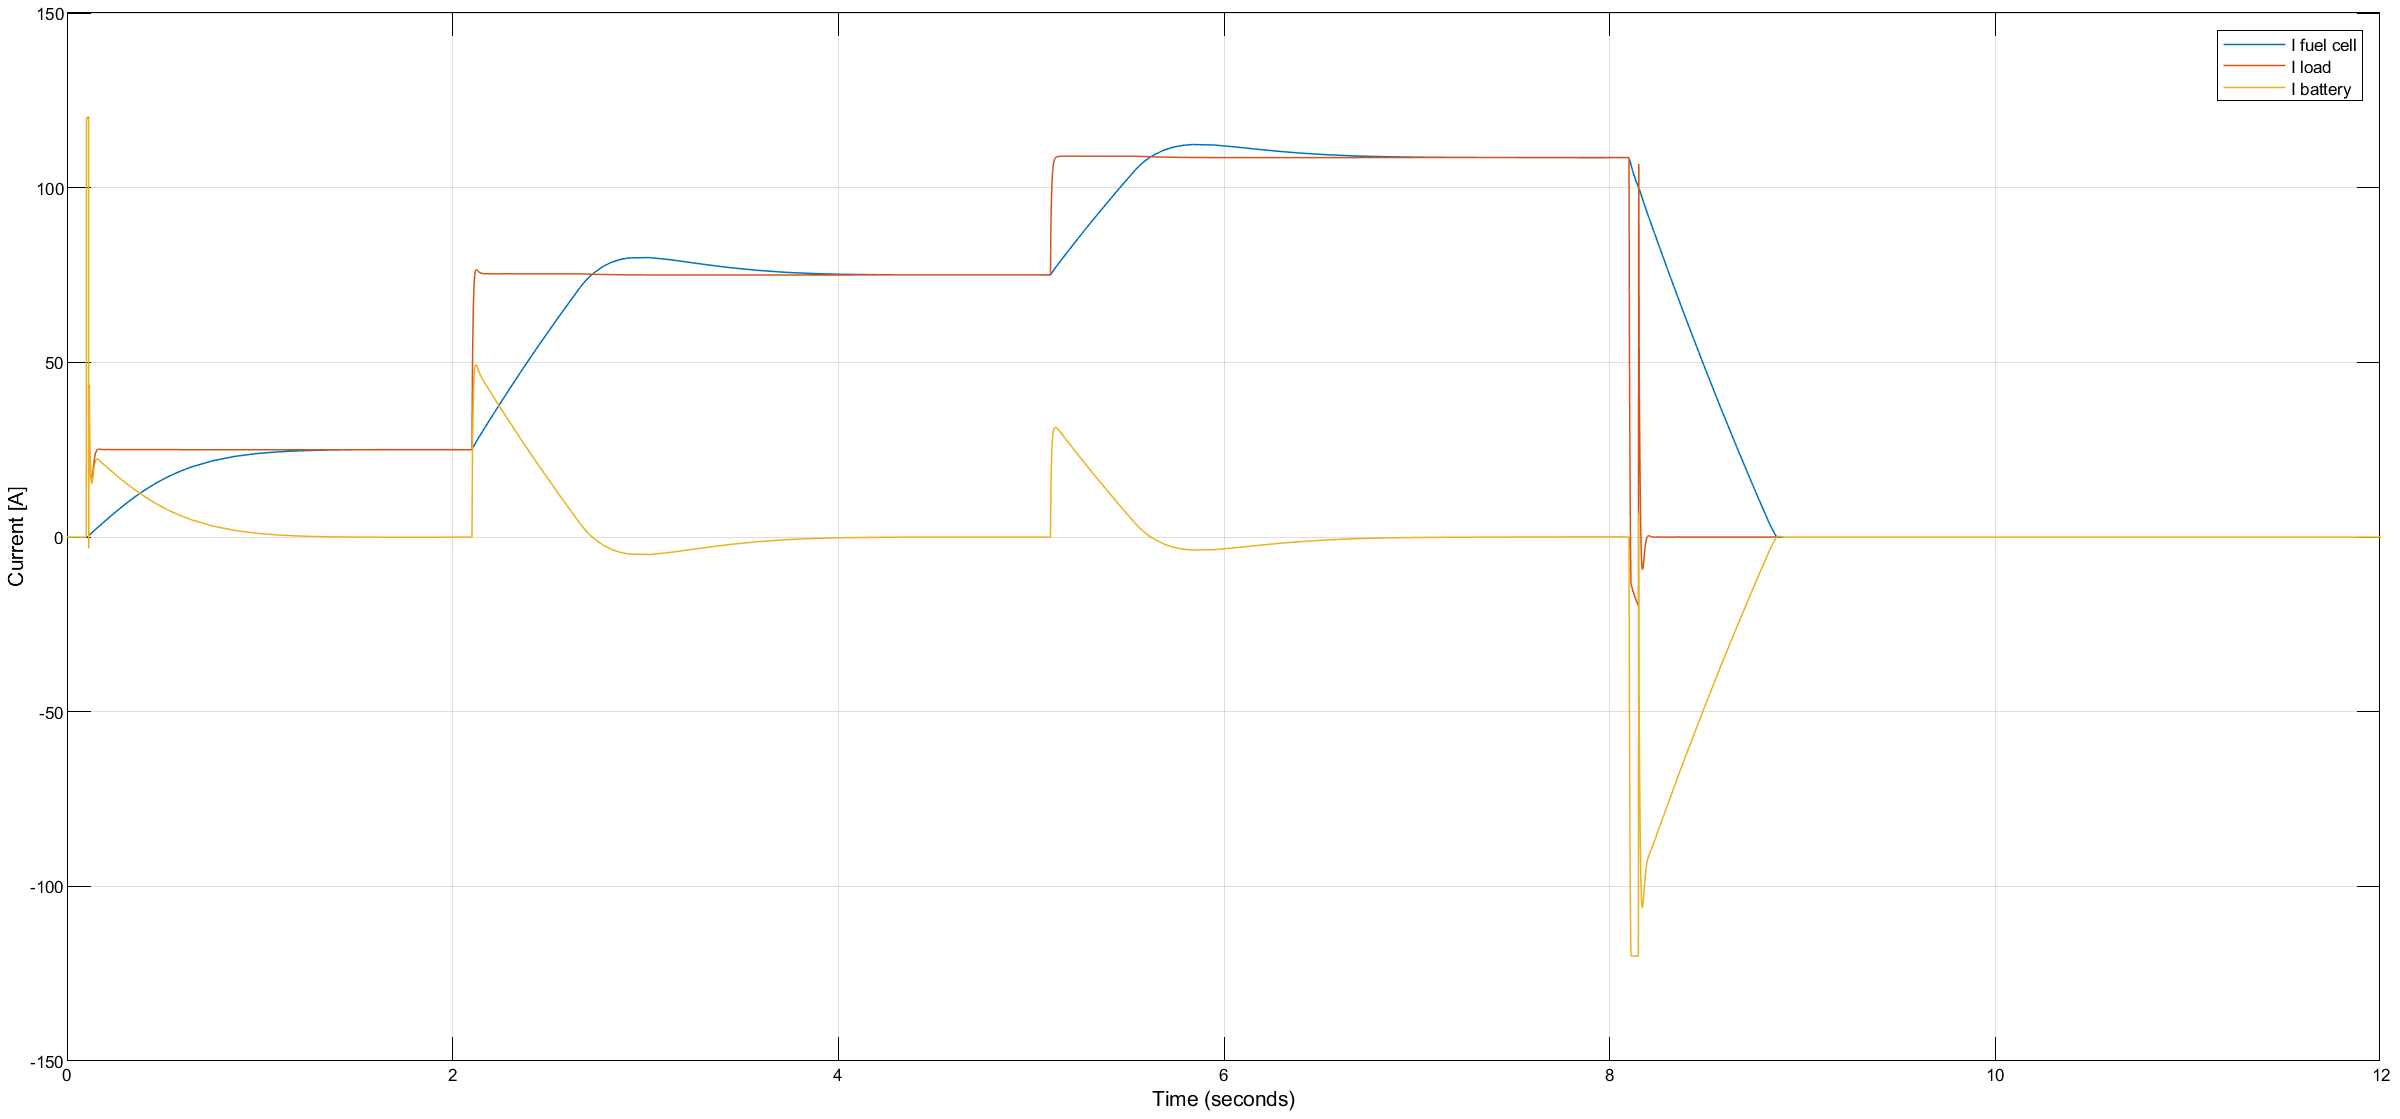
\includegraphics[width=1\linewidth]{img/simulación/e_corrientes.png}
    \caption{Corrientes del sistema.}
    \label{fig:e_corrientes}
\end{figure}

En la figura (\ref{fig:e_voltajes}) se puede observar los voltajes involucrados
en el sistema. Es posible notar que la carga se encuentra prácticamente en 
los 250 [V] durante toda la simulación por lo que el sistema MIMO cumple con 
su propósito. Por otro lado dado que los voltajes tanto de la celda de 
combustible y la batería son actuadores estos cambian de manera prácticamente
instantanea frente a los cambios producidos en la carga, pero es posible notar
que la celda de combustible se satura en 450 [V].

\begin{figure}[H]
    \centering
    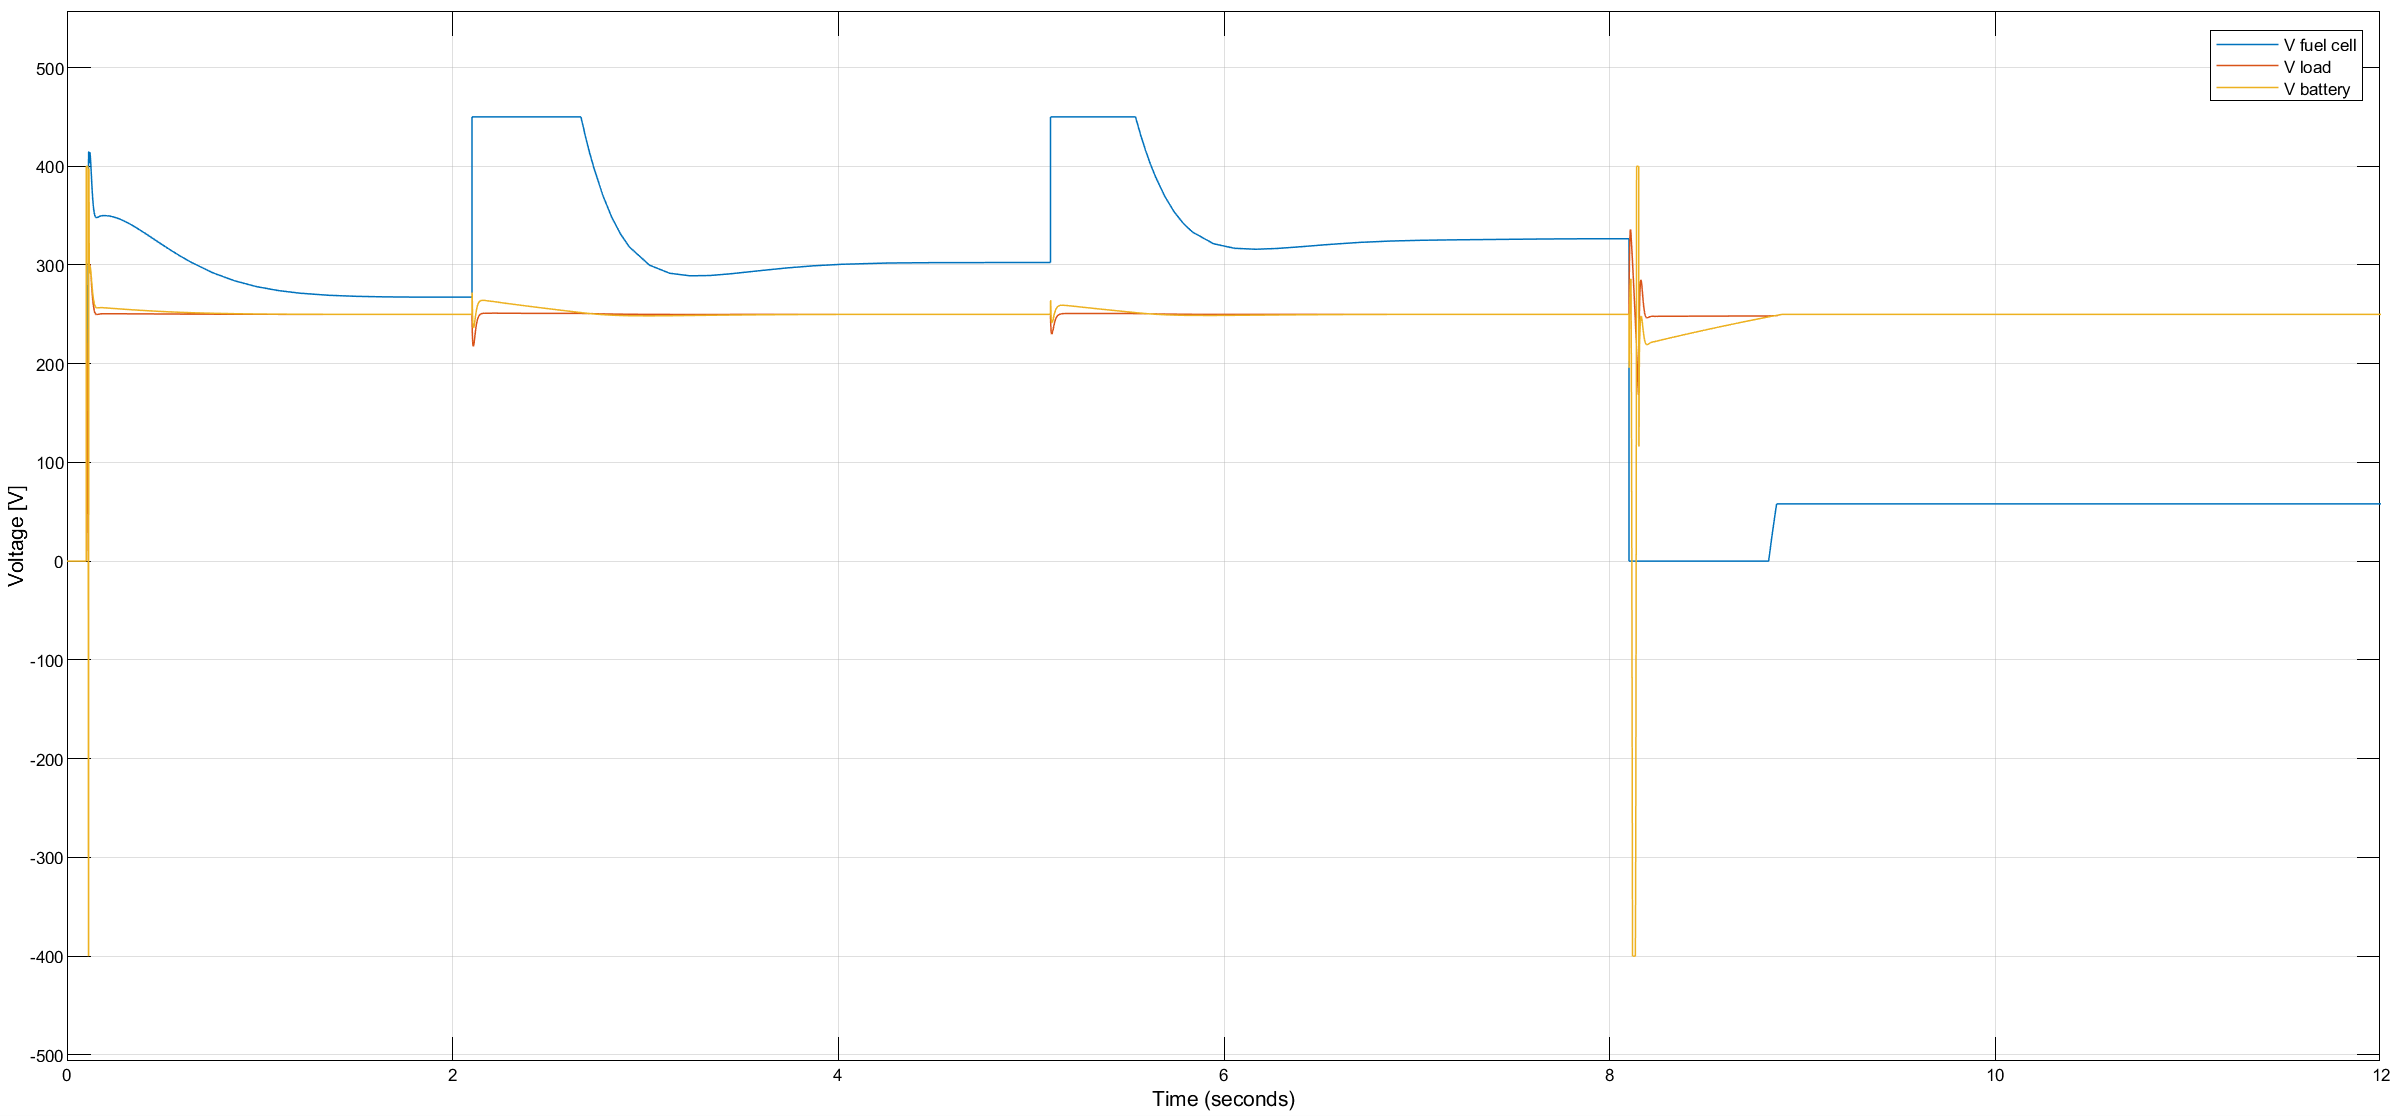
\includegraphics[width=1\linewidth]{img/simulación/e_voltajes.png}
    \caption{Voltajes del sistema.}
    \label{fig:e_voltajes}
\end{figure}

Luego en la figura (\ref{fig:e_voltajes_zoom}) se puede observar que el 
voltaje de la celda de combustible se satura en -400 y 400 [V] cuando se
desconecta la carga.

\begin{figure}[H]
    \centering
    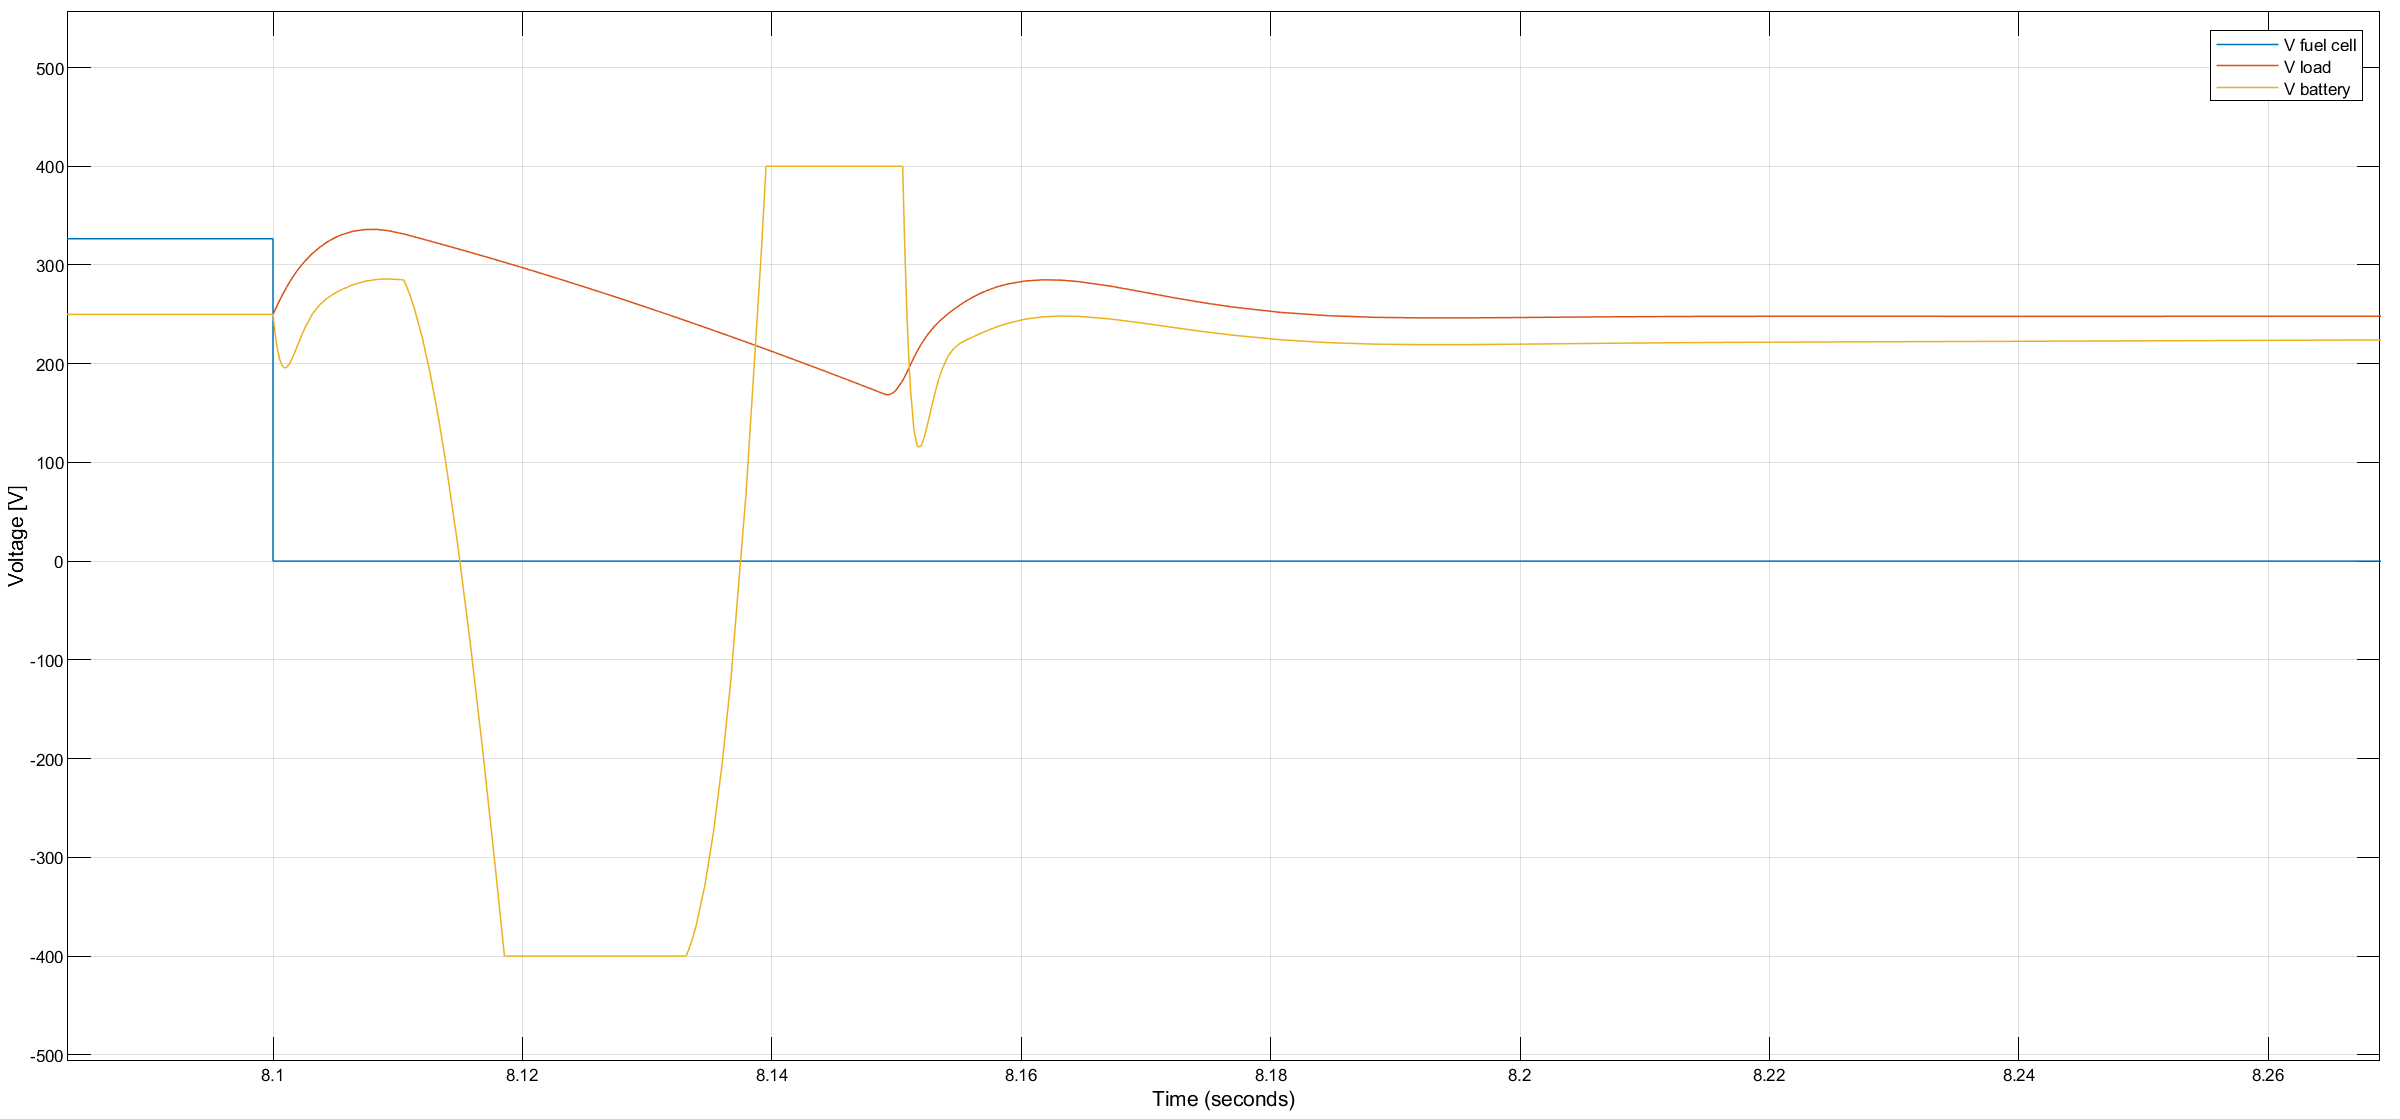
\includegraphics[width=1\linewidth]{img/simulación/e_voltajes_zoom.png}
    \caption{Voltajes con zoom.}
    \label{fig:e_voltajes_zoom}
\end{figure}



%==================================== f) ====================================
\subsection{\textit{Simulación con dos cambios en la carga}}
%==================================== f) ====================================

\begin{table}[H]
    \centering
    \begin{tabular}{|c|c|}
    \hline
    \textbf{Inicialización del sistema} & \textbf{Resistencia de carga} \\
    \hline
    $0 \leq t < 2$ (seg.) & $R_L = 10\,\Omega$ \\
    \hline
    $2 \leq t < 5$ (seg.) & Resistencia de carga total de $R_L = 2.3\,\Omega$ \\
    \hline
    $5 \leq t < 8$ (seg.) & La carga total se desconecta y $R_L \rightarrow \infty$ \\
    \hline
\end{tabular}
\caption{Escenario con dos perturbaciones de carga.}
\label{tab:f}
\end{table}


\begin{figure}[H]
    \centering
    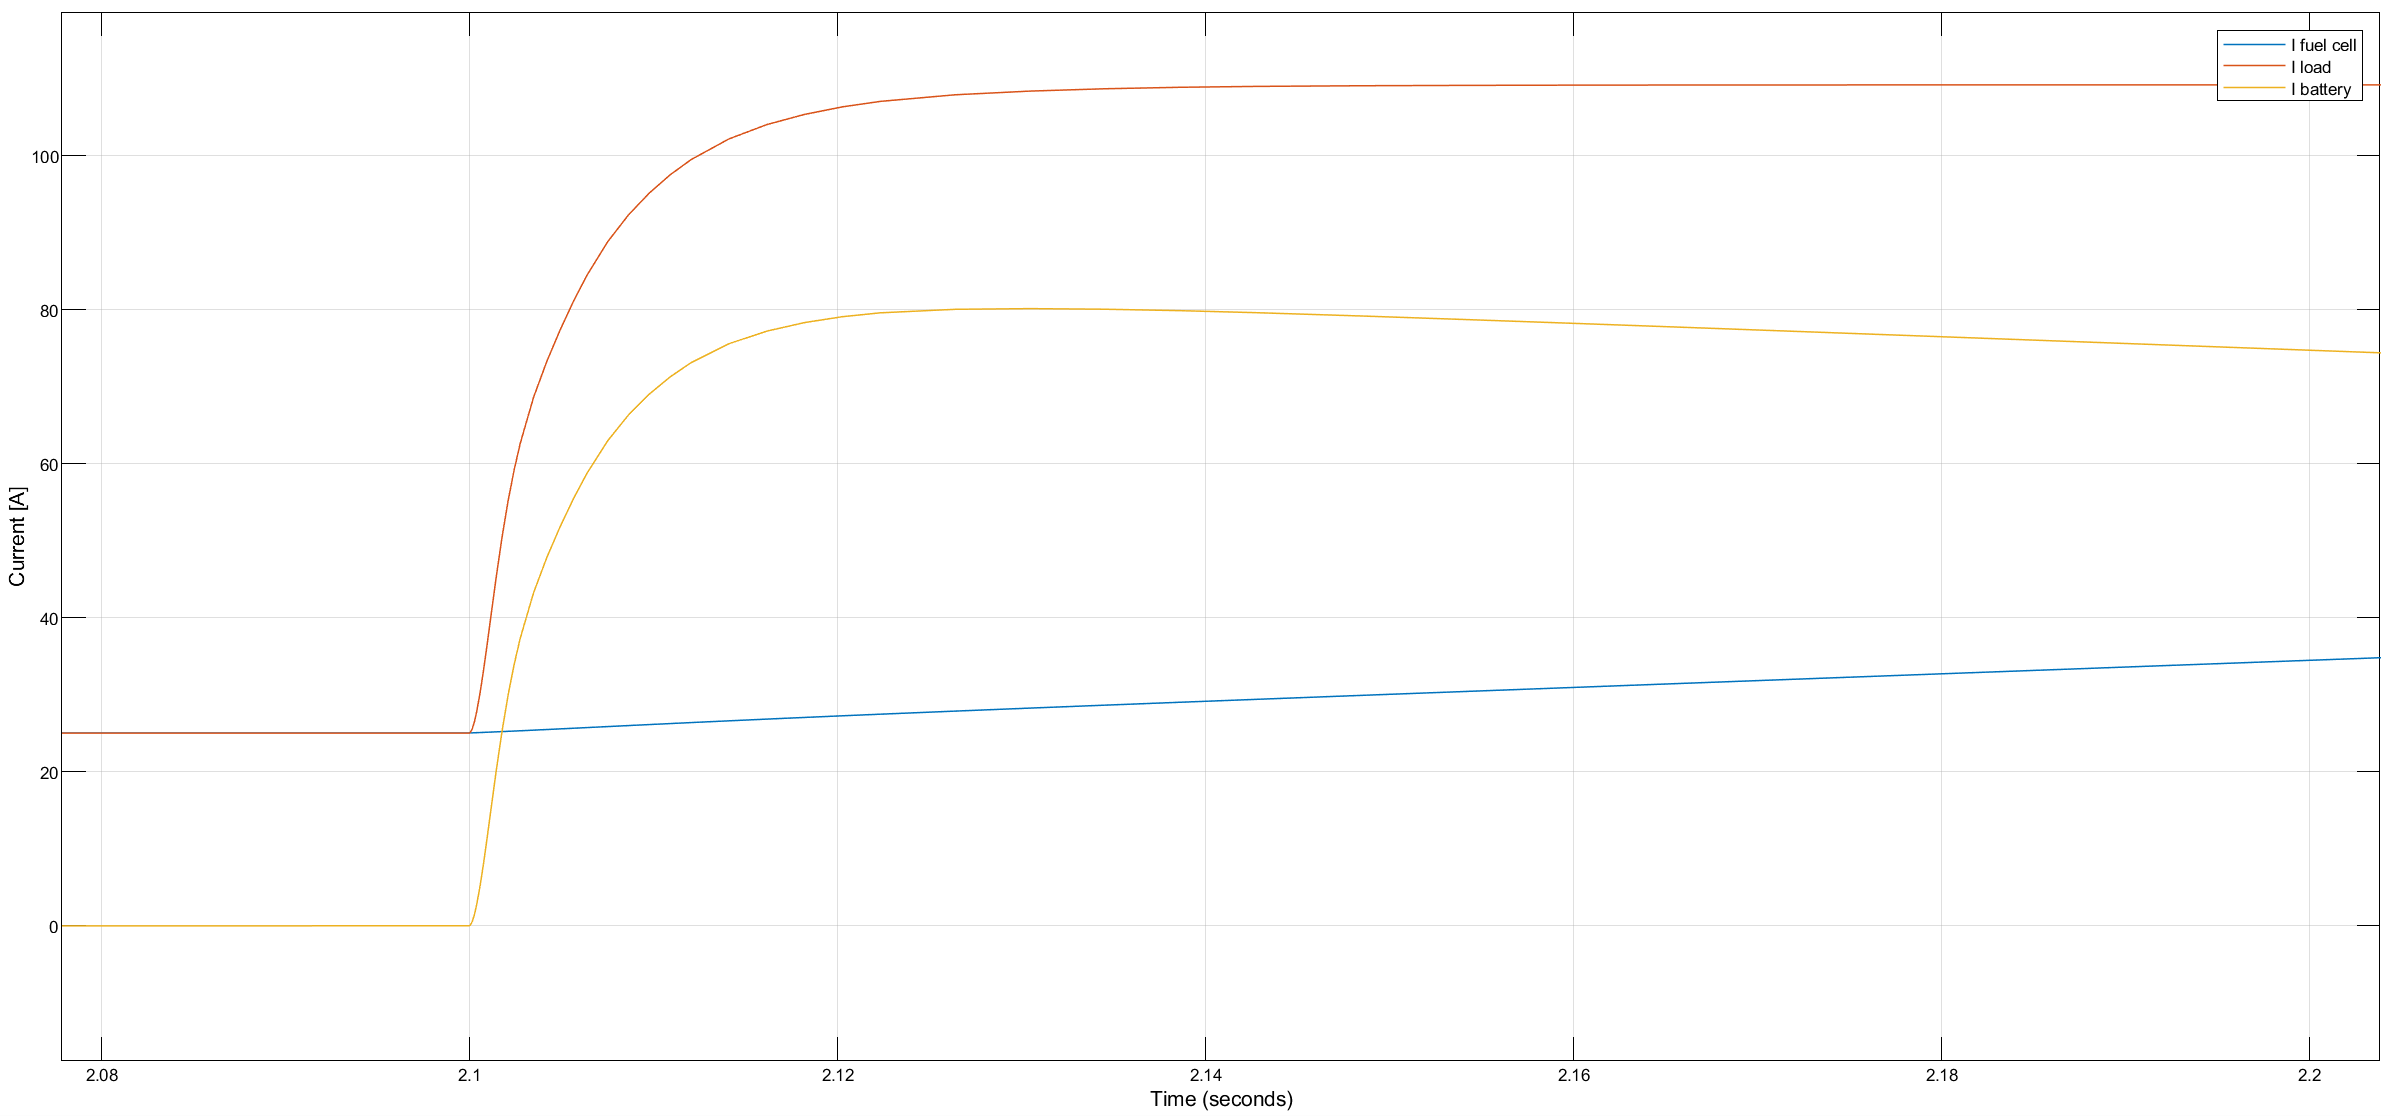
\includegraphics[width=1\linewidth]{img/simulación/f_corriente_1.98-2.1.png}
    \caption{Corriente entre 1.98 y 2.1 segundos.}
    \label{fig:f_corriente_1.98-2.1}
\end{figure}

\begin{figure}[H]
    \centering
    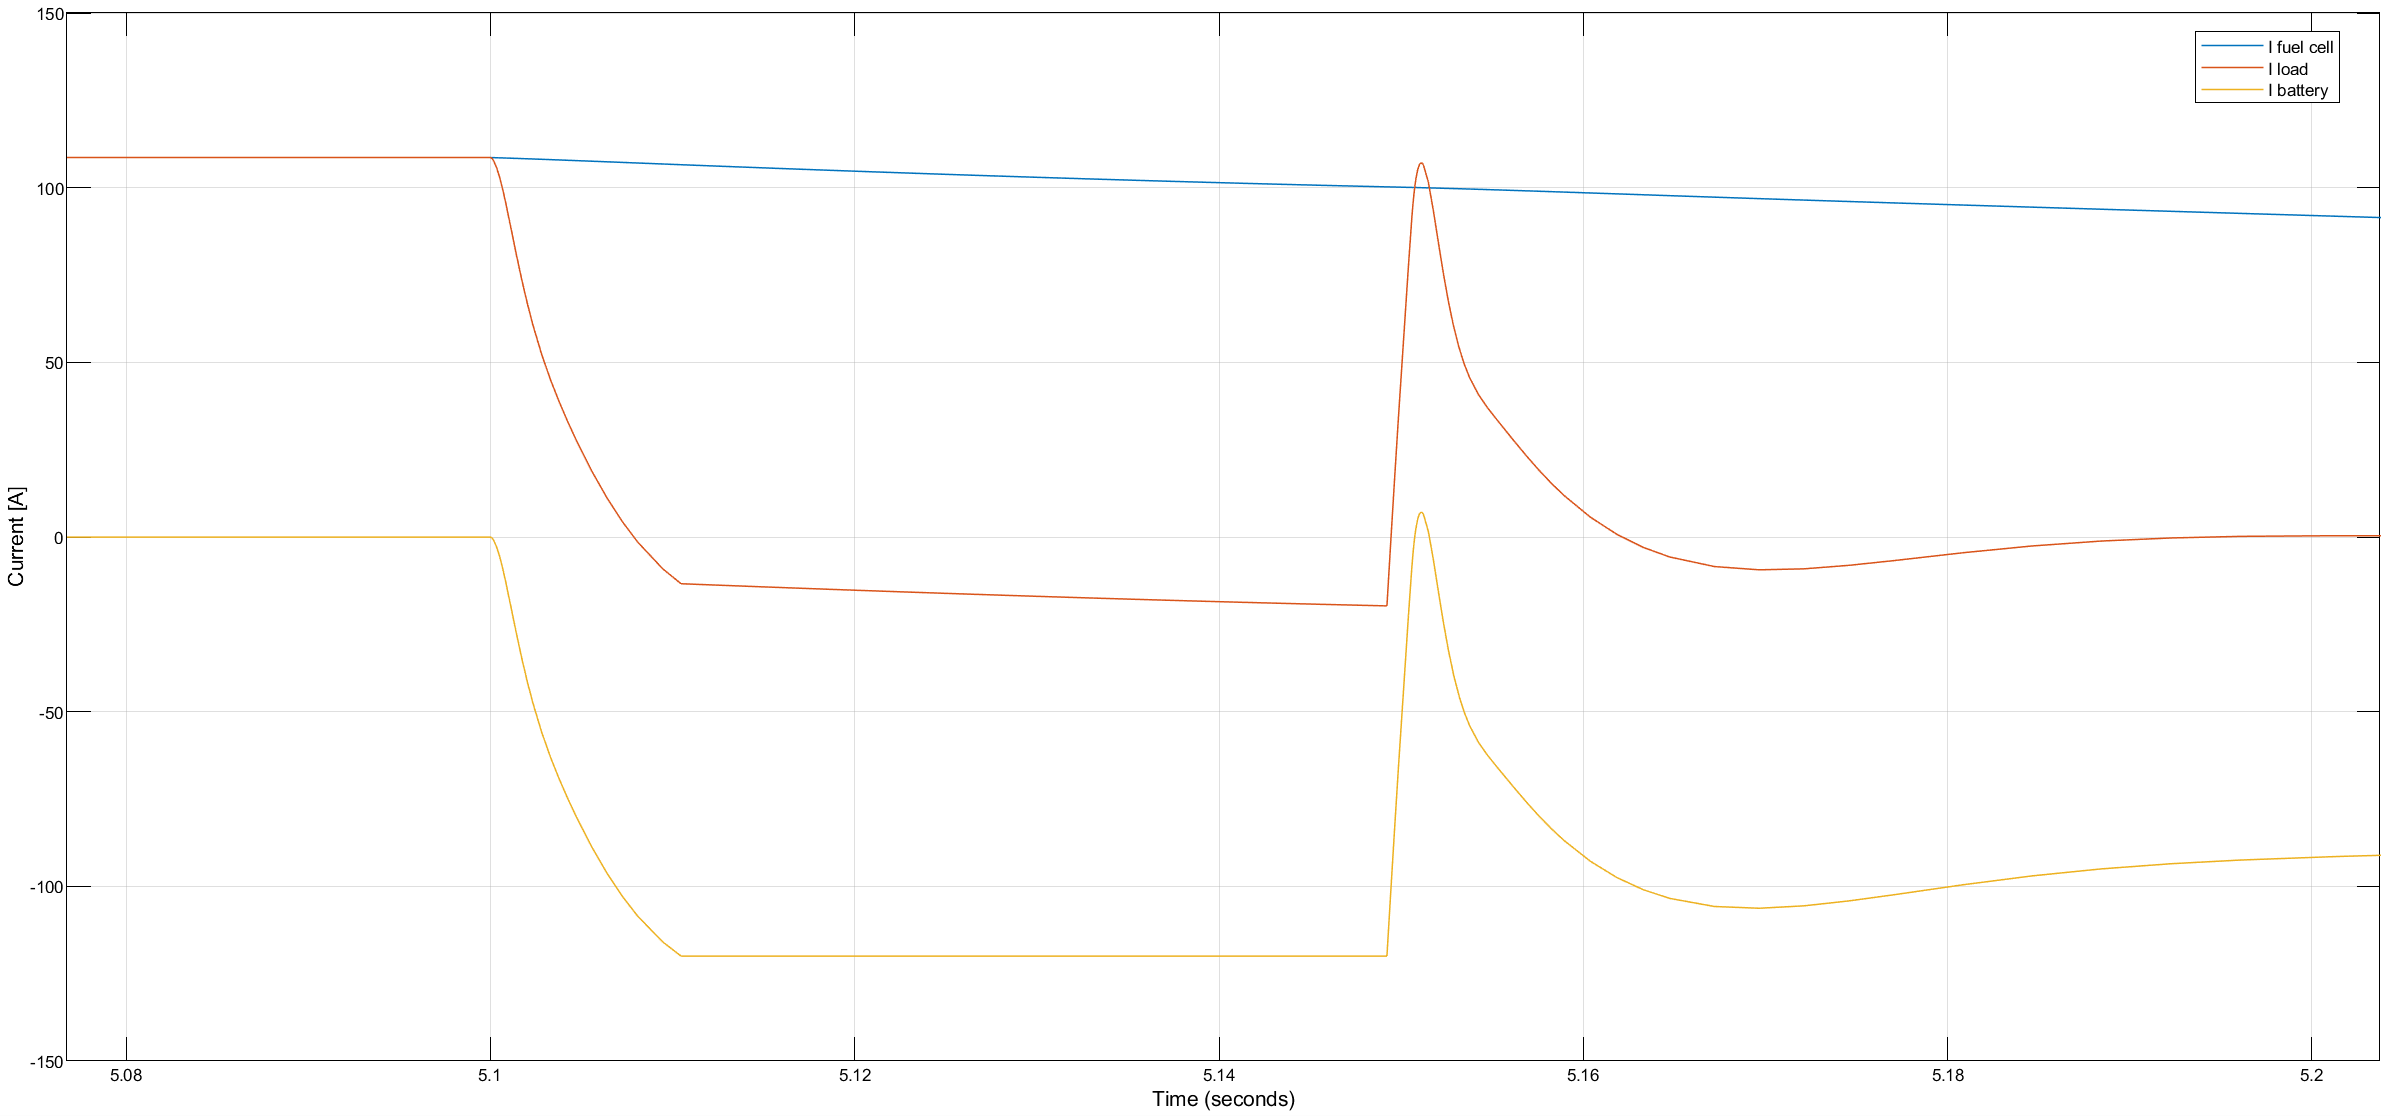
\includegraphics[width=1\linewidth]{img/simulación/f_corriente_4.98-5.1.png}
    \caption{Corriente entre 4.98 y 5.1 segundos.}
\label{fig:f_corriente_4.98-5.1}
\end{figure}

Se puede notar que la batería no suministraba corriente antes de la perturbación. 
Después de ocurrir el cambio de resistencia $R_L$ las corrientes de la \textit{fuel cell} y de
la batería aumentan para poder compensar con la caida de tensión que inevitablemente ocurre. 
Luego de dicha perturbación la corriente usada por la batería converge a cero. 

\begin{figure}[H]
    \centering
    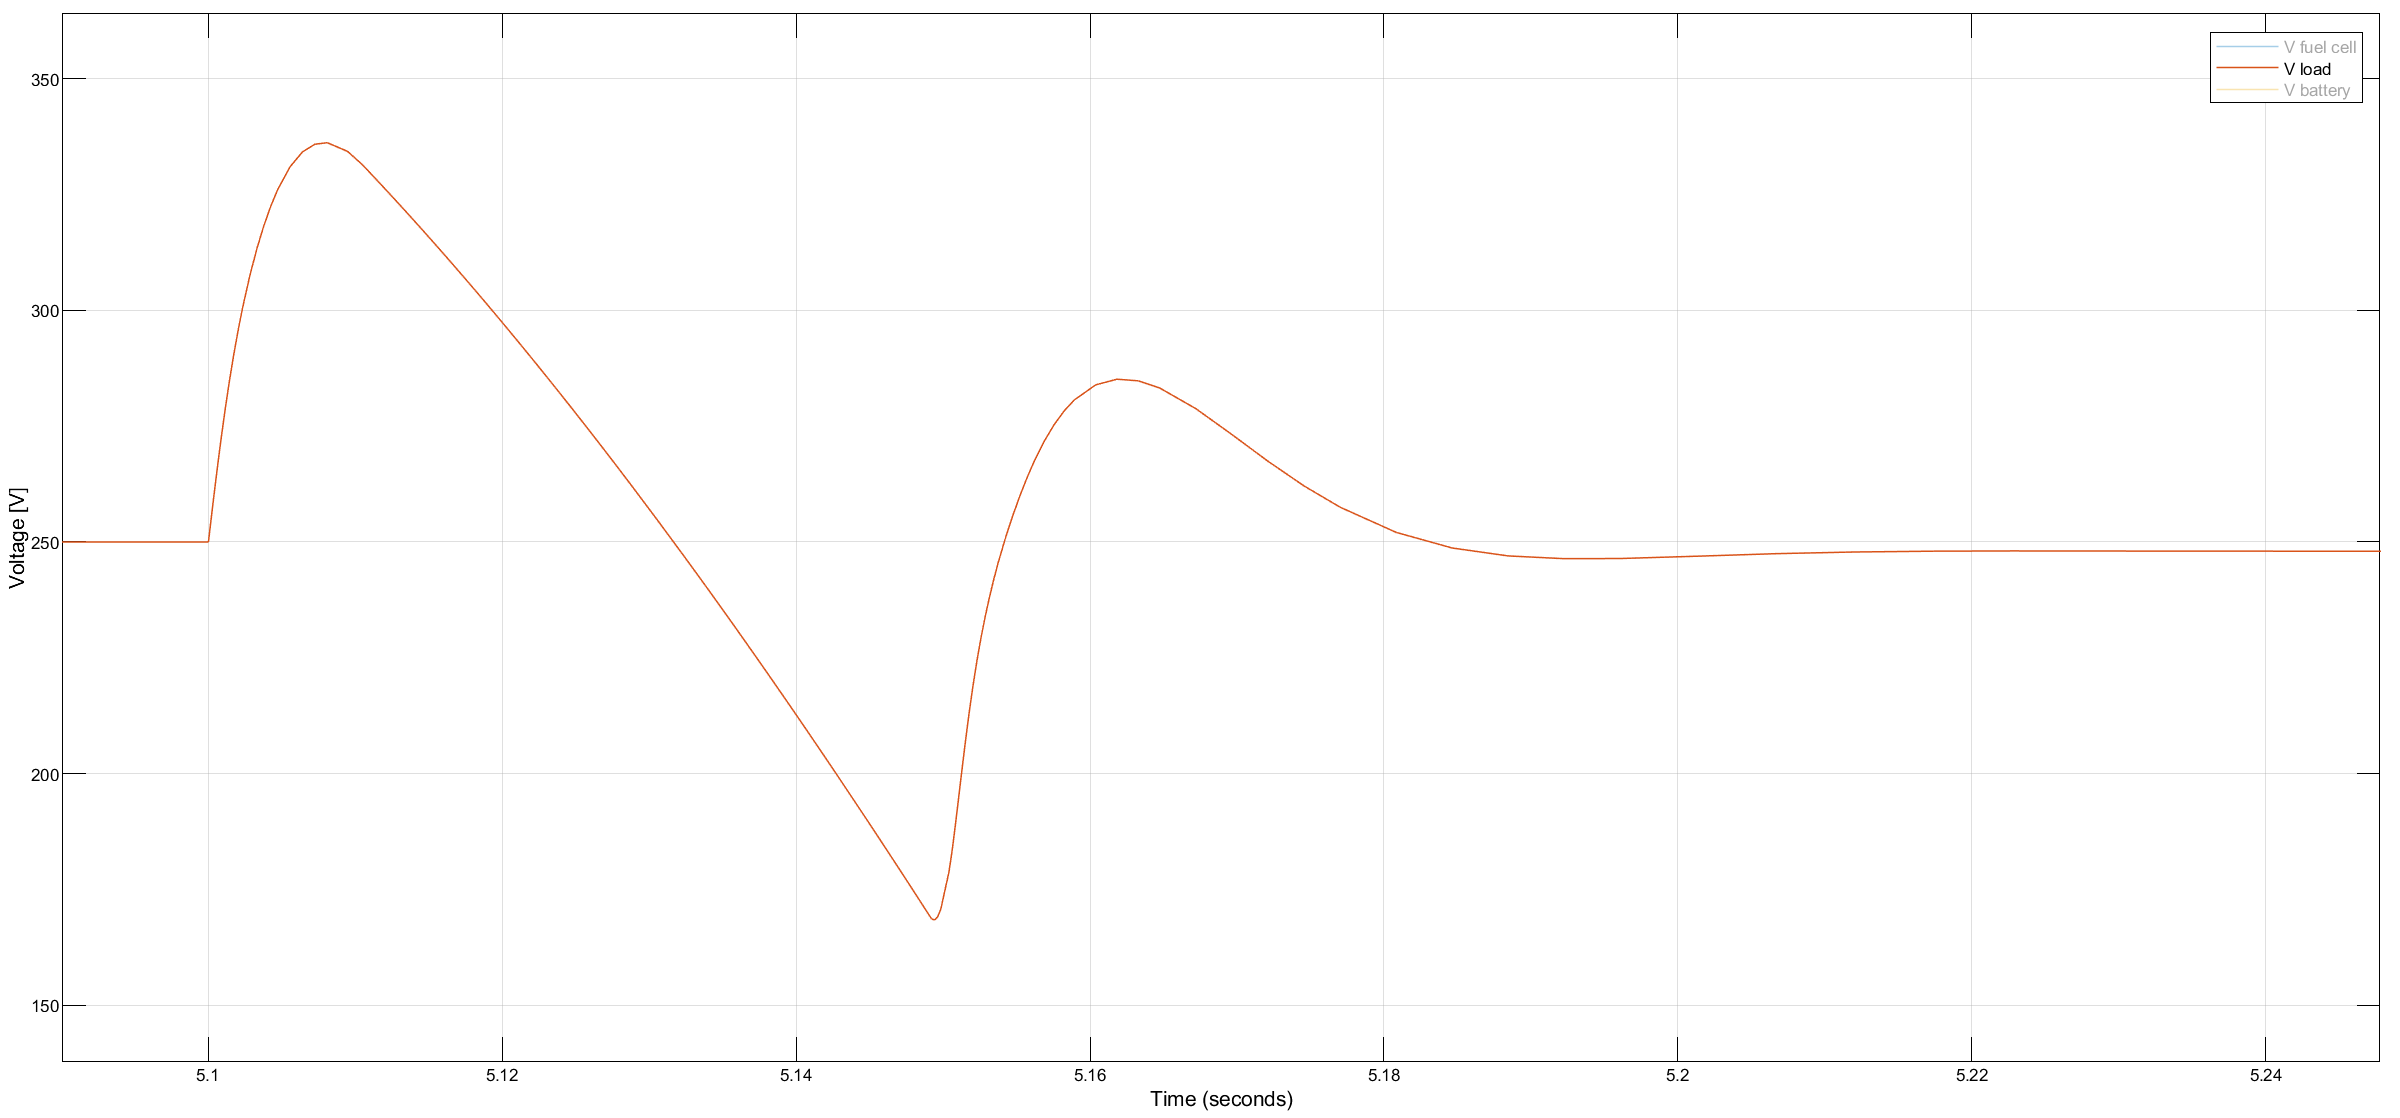
\includegraphics[width=1\linewidth]{img/simulación/f_maximosobrepaso.png}
    \caption{Máximo sobrepaso del sistema.}
\label{fig:f_maximosobrepaso}
\end{figure}

El voltaje de la carga más alto se alcanza cuando se desconecta la carga, como se puede observar 
en la figura (\ref{fig:f_maximosobrepaso}), llega hasta unos 340 [V] aproximadamente
que equivale a un sobre paso de 36\% ($\frac{340-250}{250} \cdot 100$). Y seguido de eso alcanza 
también su valor mínimo cerca de los 170 [V], pero vuelve a estar aproximadamente en 250 [V]
pasados unos 0.2 segundos.

\begin{figure}[H]
    \centering
    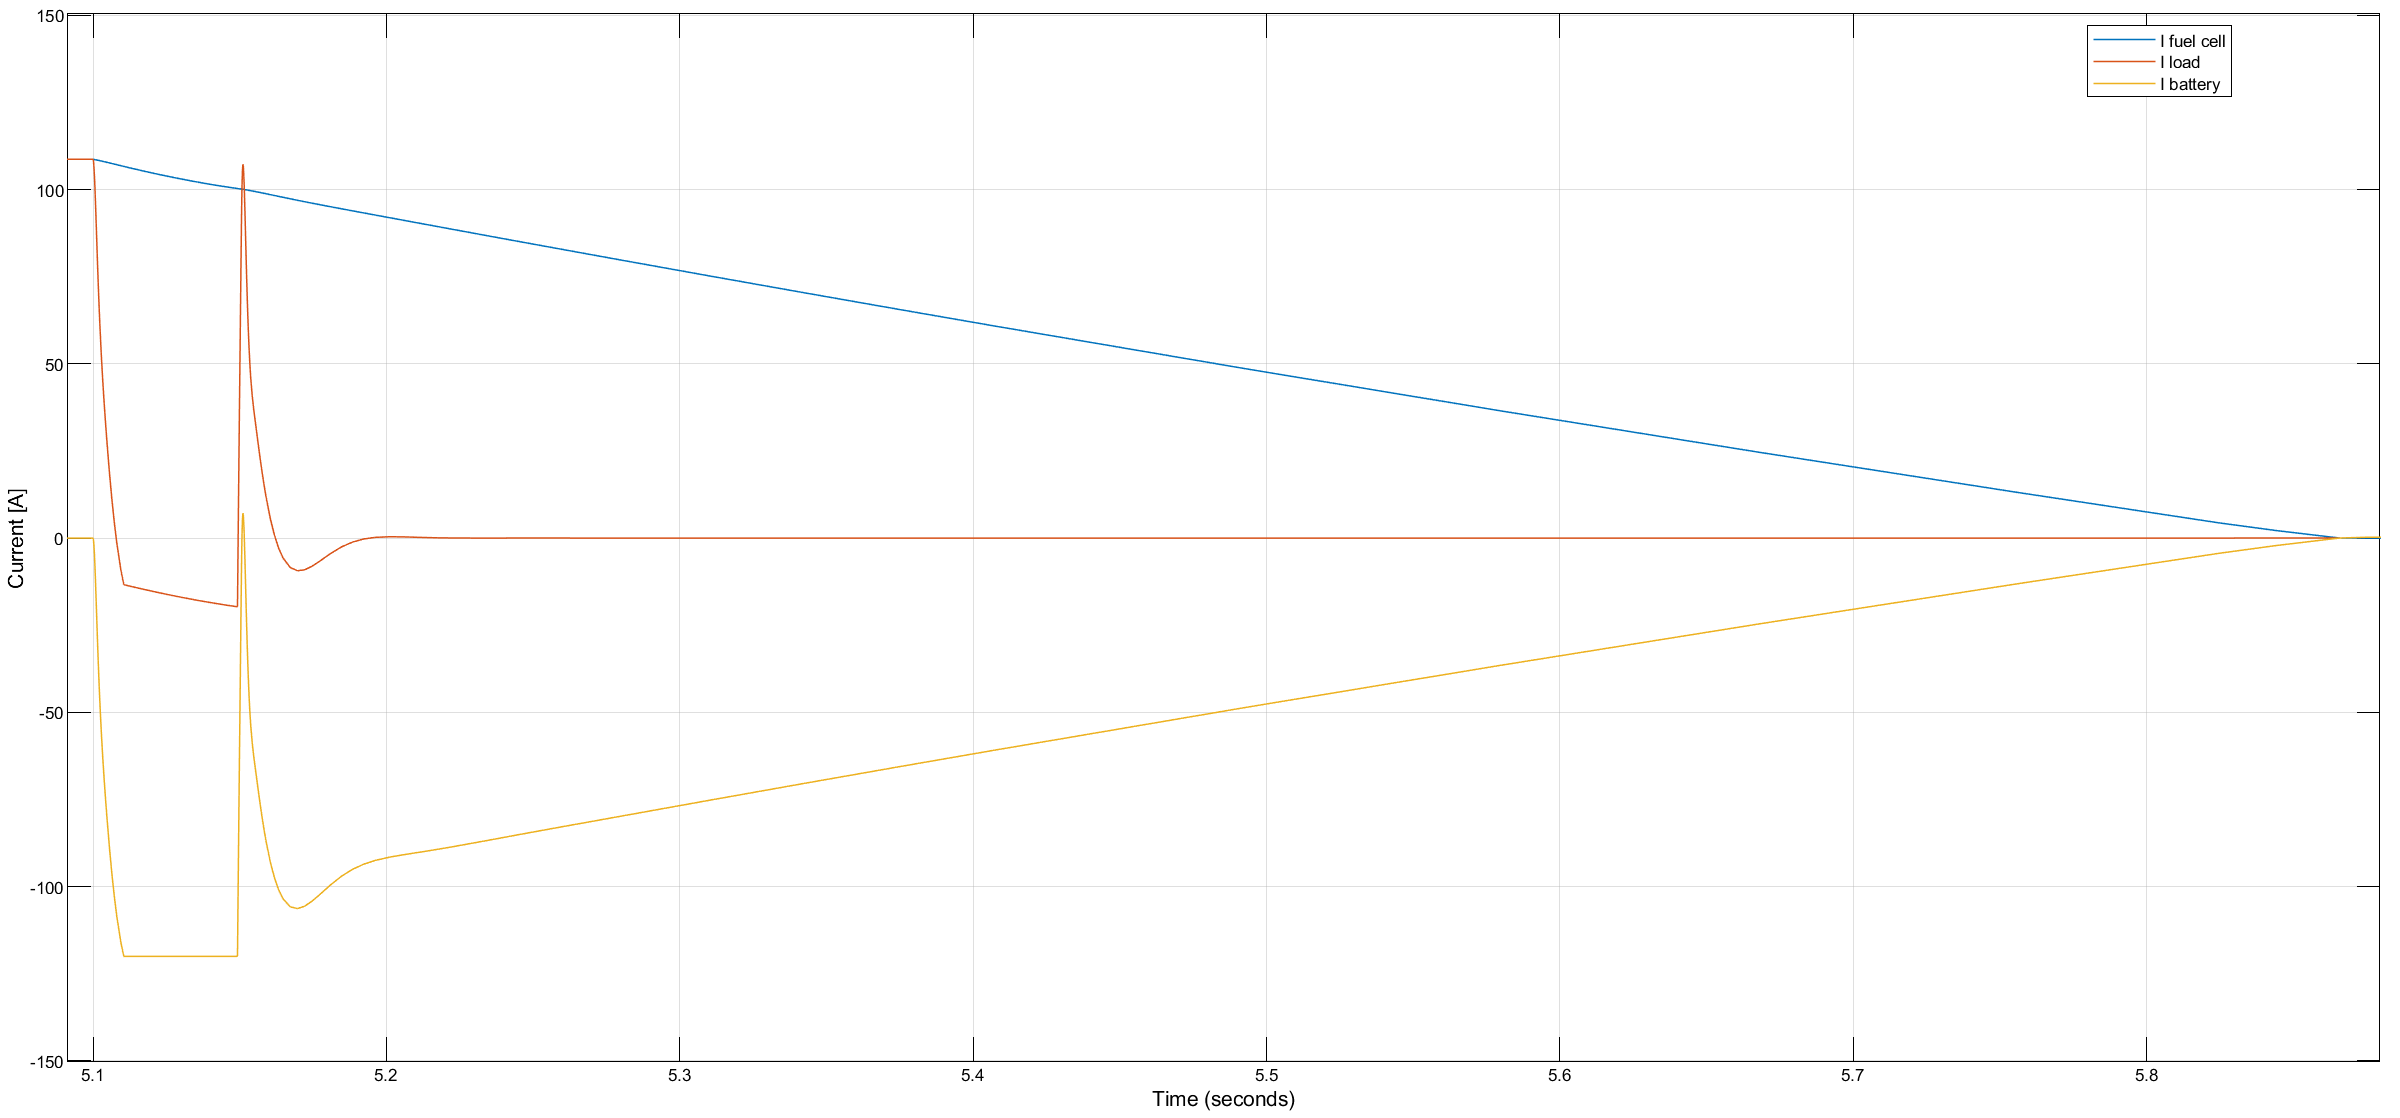
\includegraphics[width=1\linewidth]{img/simulación/f_tiempoestablecimientofuelcell.png}
    \caption{Tiempo de establecimiento de la celda de combustible.}
    \label{fig:f_tiempoestablecimientofuelcell}
\end{figure}

%==================================== g) ====================================


\begin{figure}[H]
    \centering
    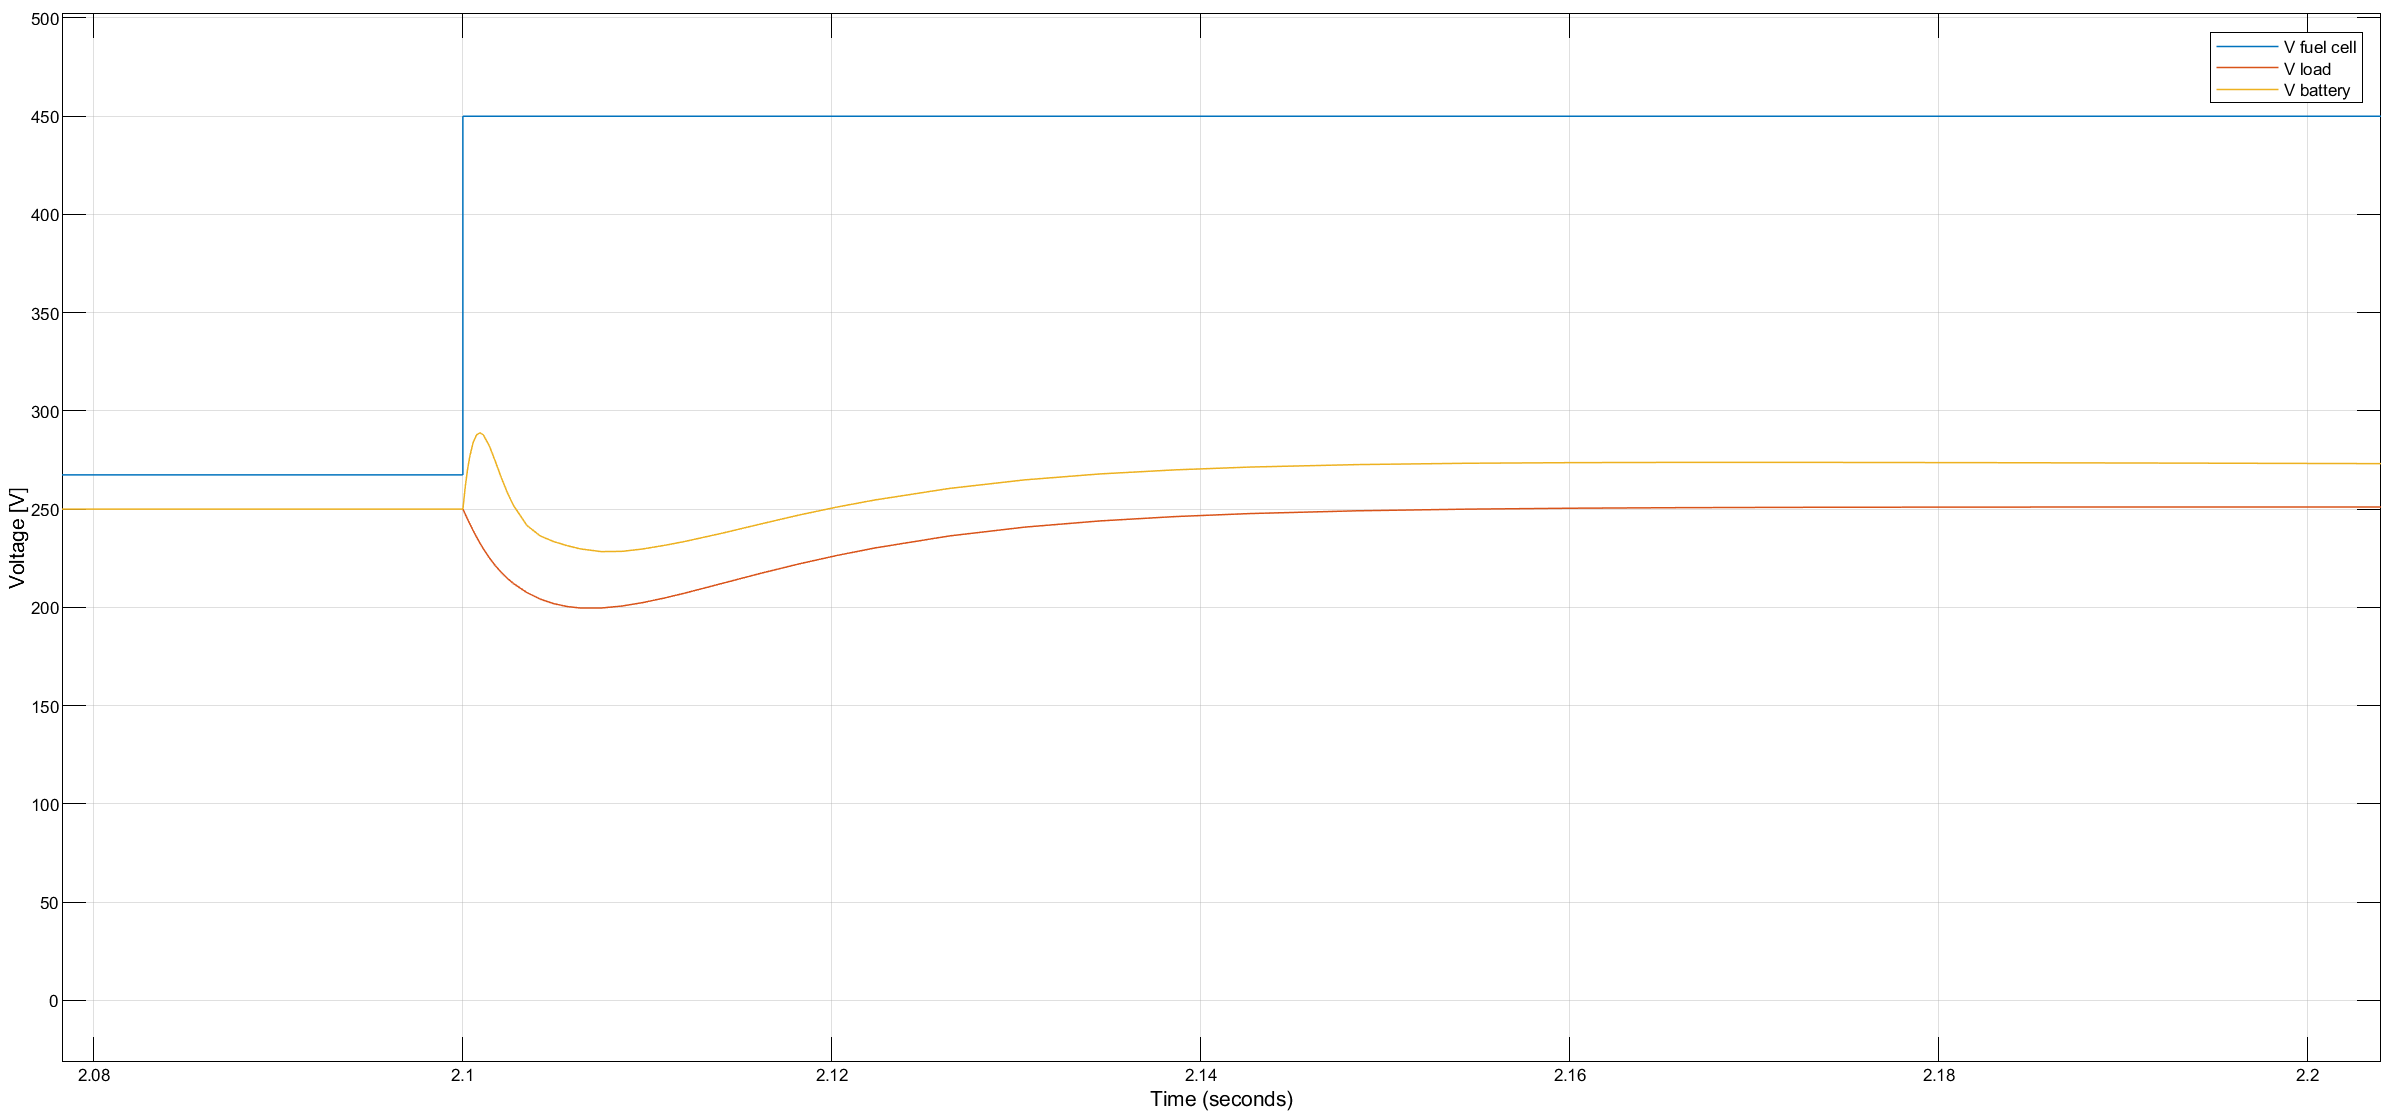
\includegraphics[width=1\linewidth]{img/simulación/g_volt1.98-2.1.png}
    \caption{Voltaje entre 1.98 y 2.1 segundos.}
    \label{fig:g_volt1.98-2.1}
\end{figure}

\begin{figure}[H]
    \centering
    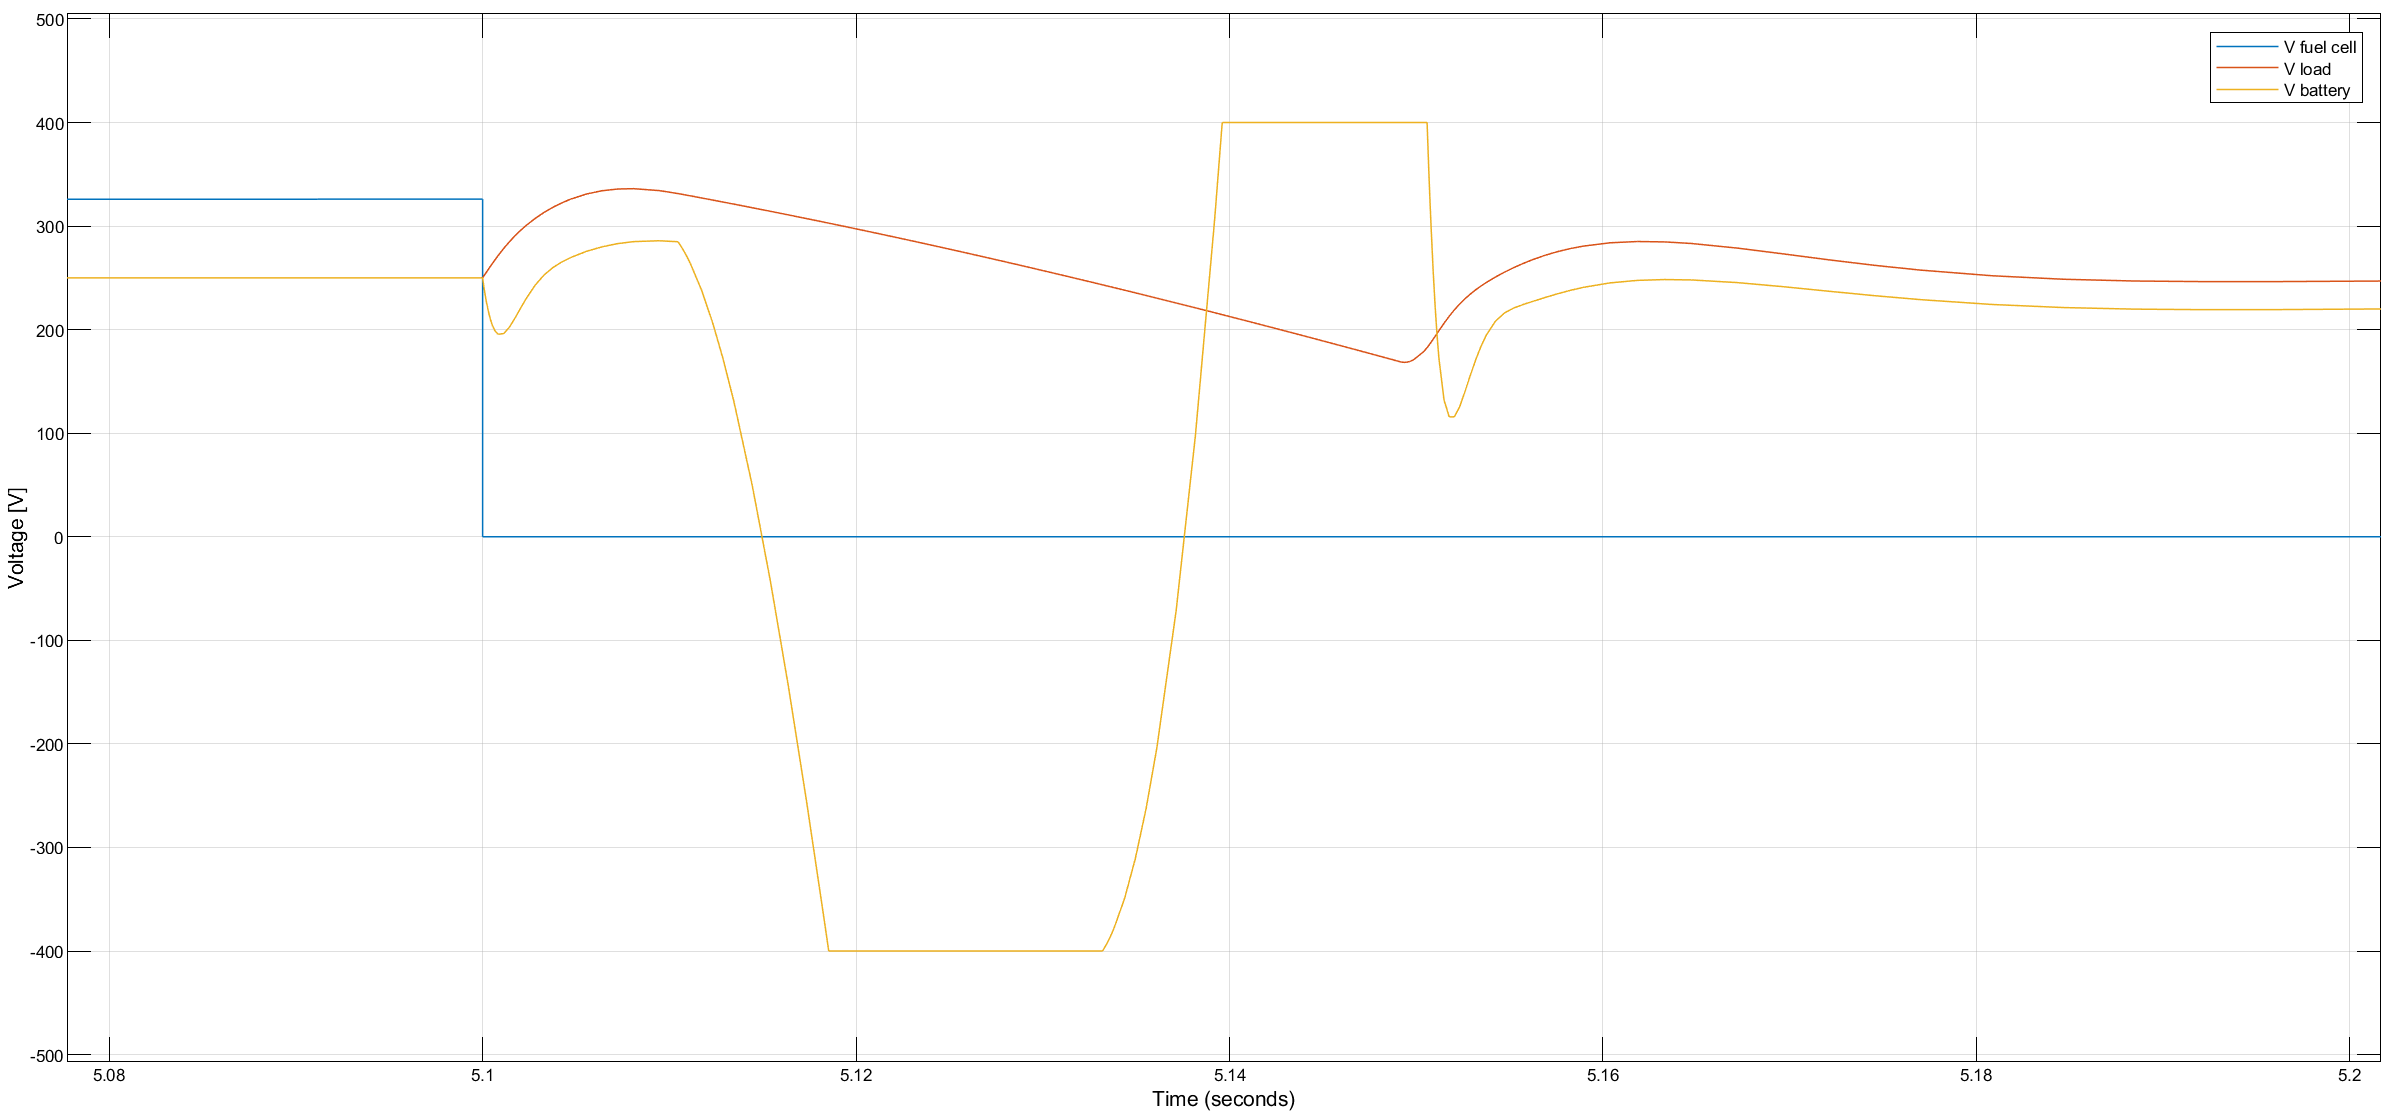
\includegraphics[width=1\linewidth]{img/simulación/g_volt4.98-5.1.png}
    \caption{Voltaje entre 4.98 y 5.1 segundos.}
    \label{fig:g_volt4.98-5.1}
\end{figure}

%==================================== h) ====================================
\subsection{\textit{Sistema sin Anti-Winding Up}}
%==================================== h) ====================================

\begin{figure}[H]
    \centering
    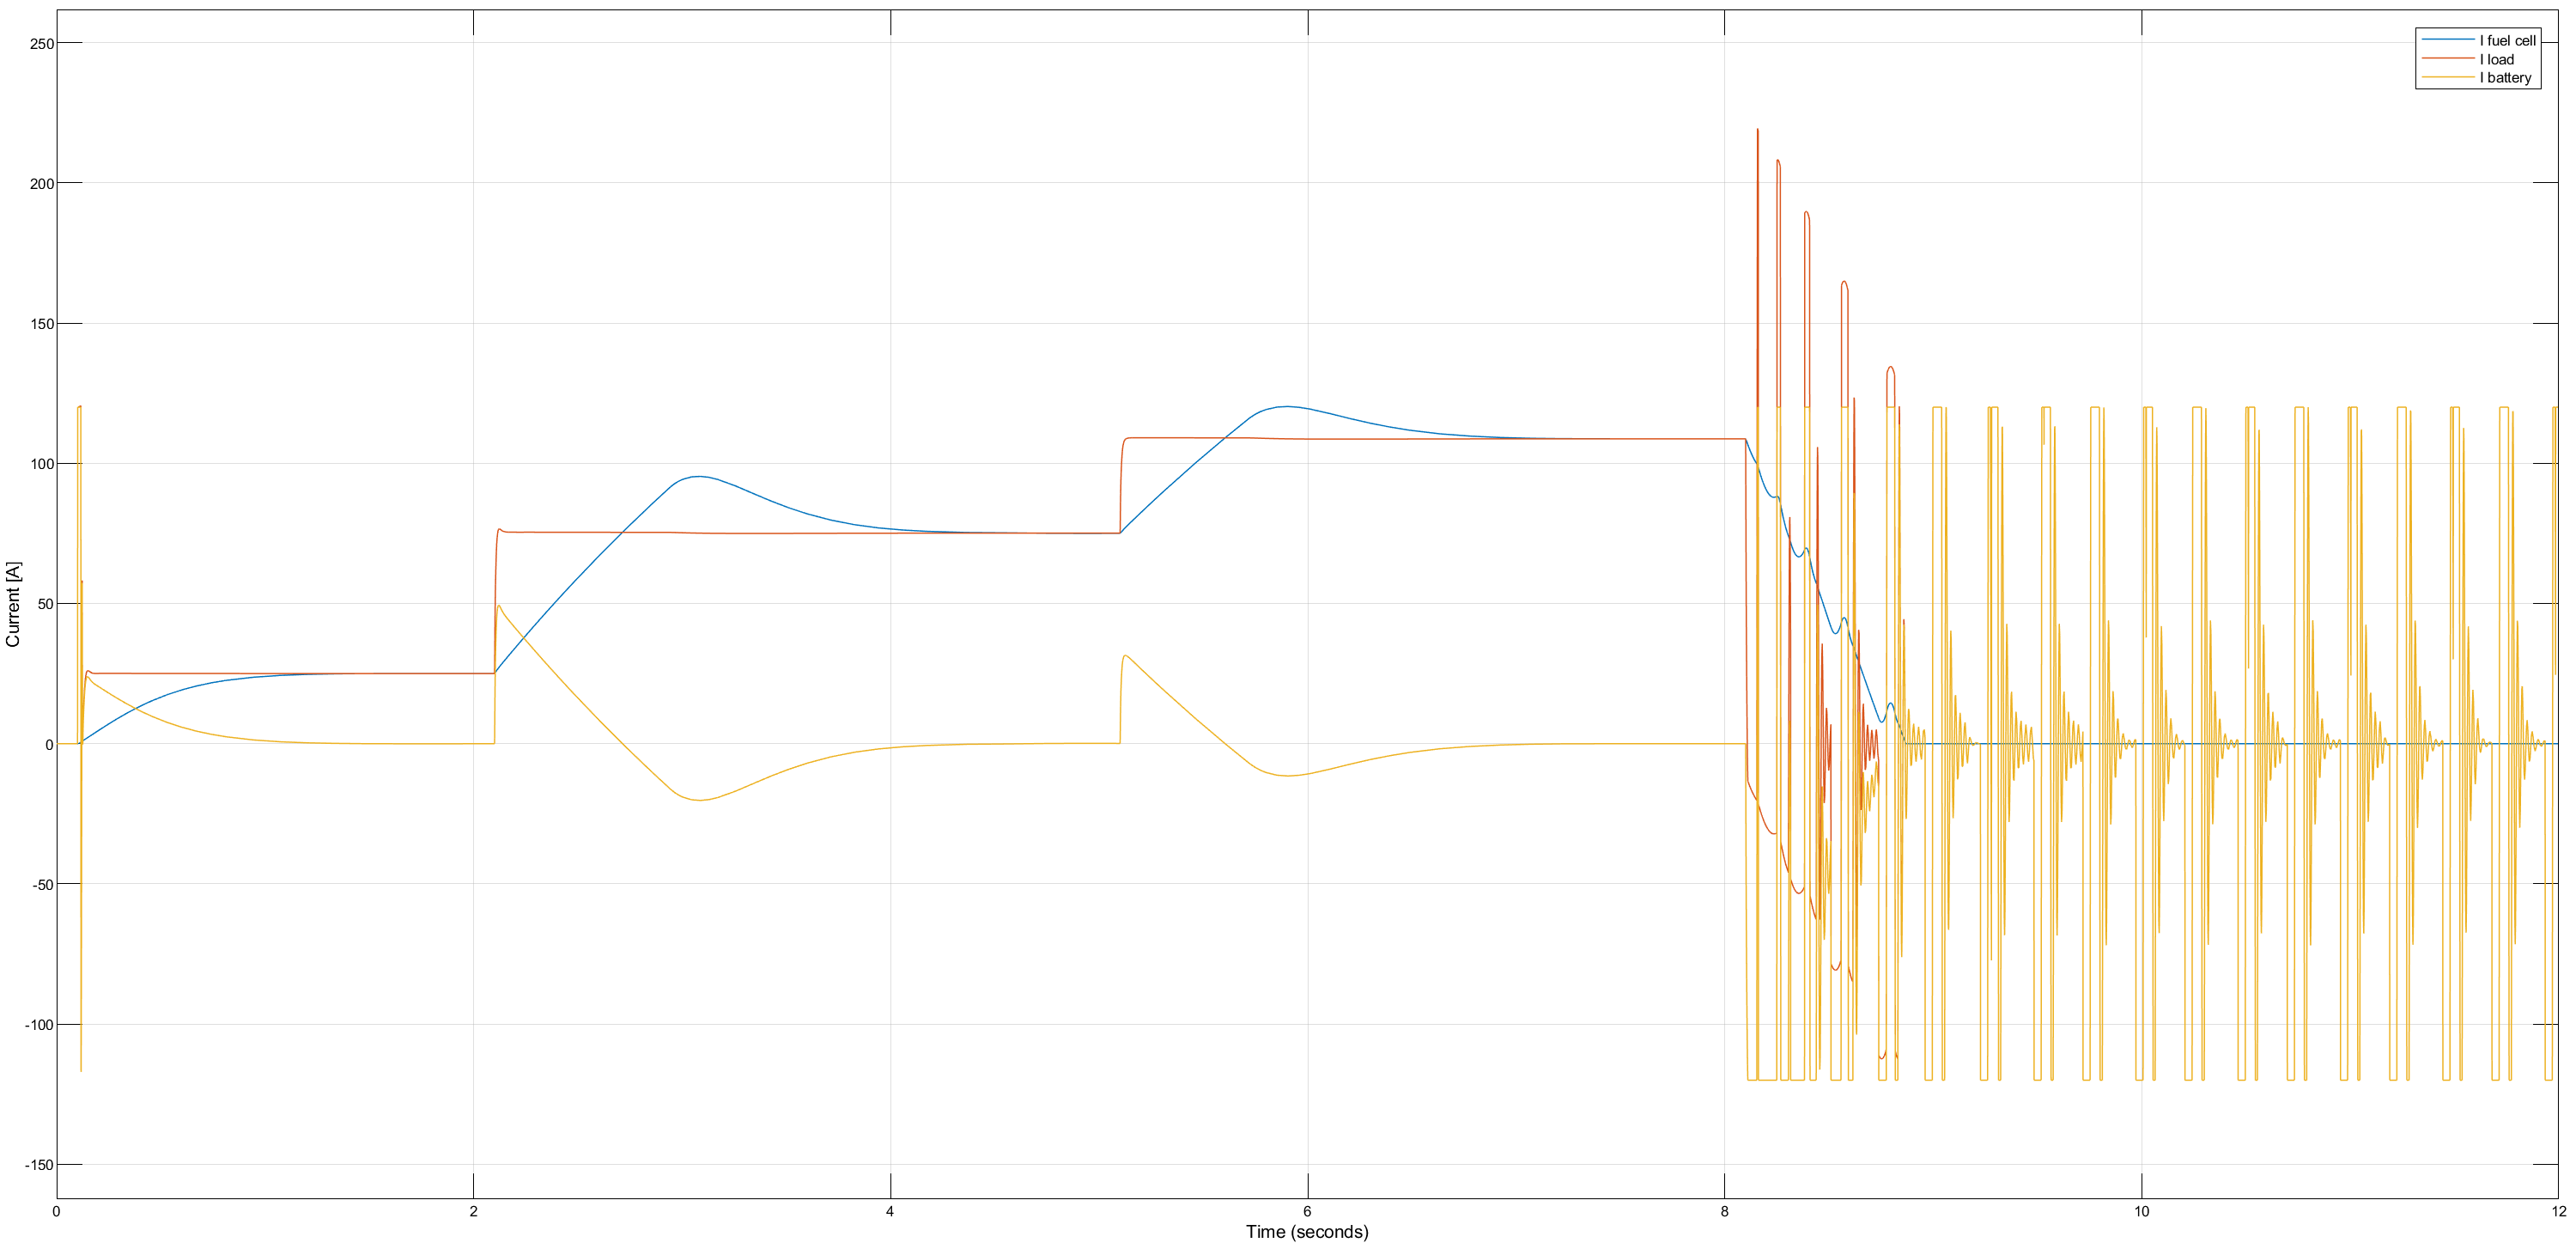
\includegraphics[width=1\linewidth]{img/simulación/h_corrientes.png}
    \caption{Corrientes del sistema en otra condición.}
    \label{fig:h_corrientes}
\end{figure}

\begin{figure}[H]
    \centering
    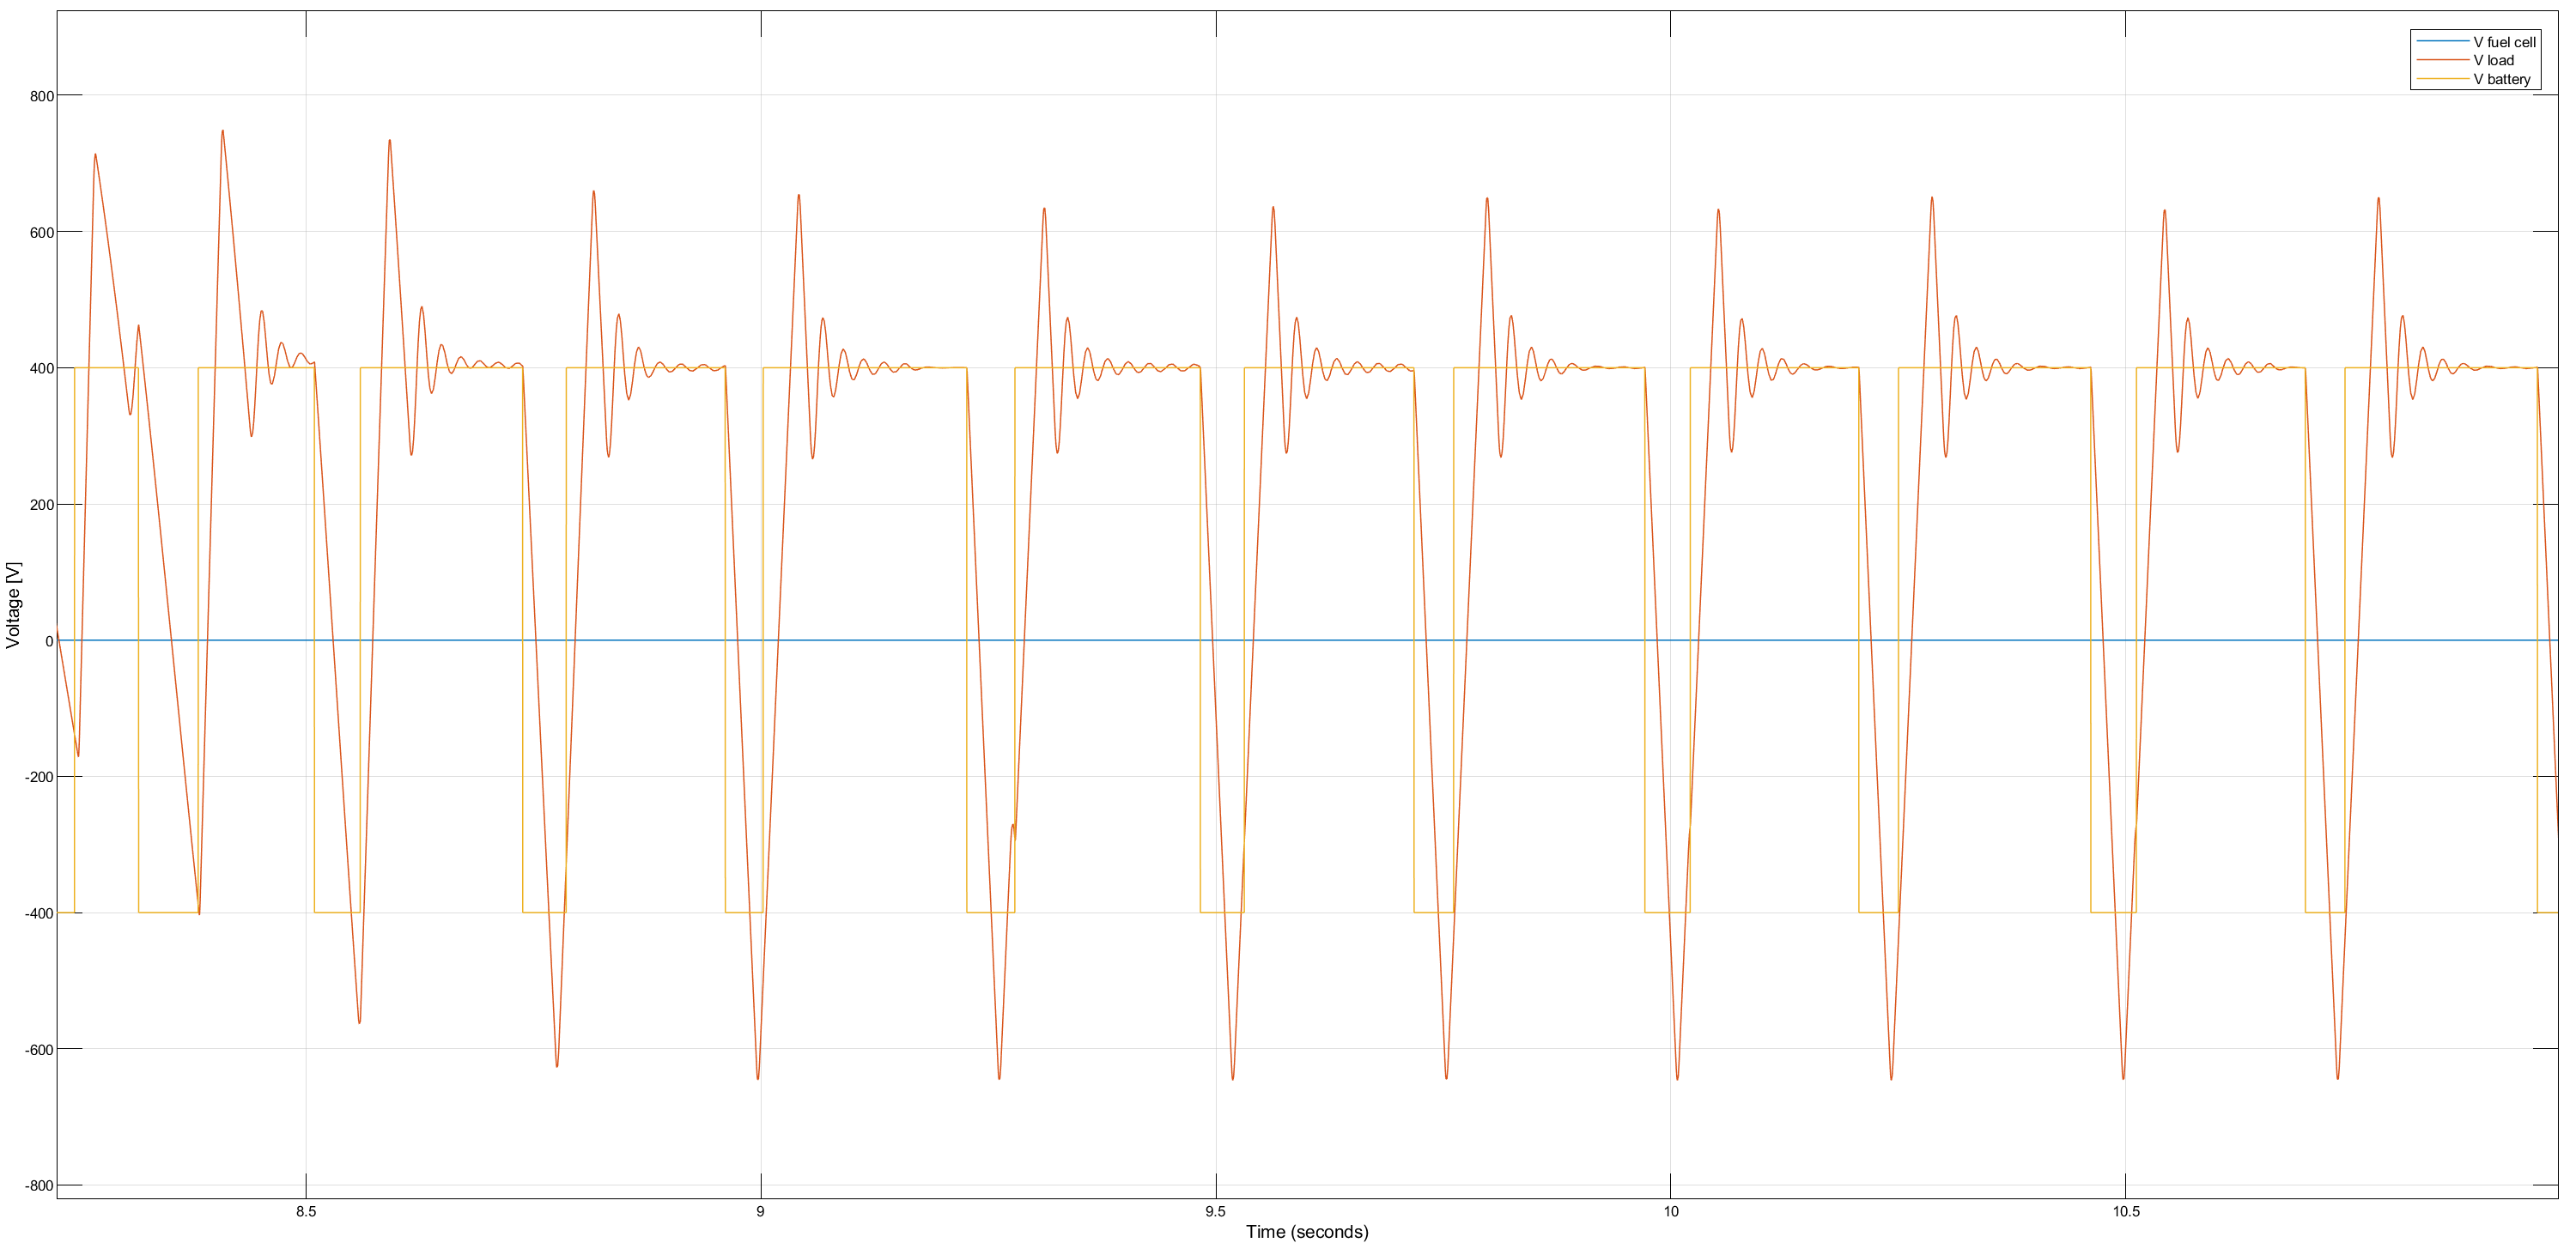
\includegraphics[width=1\linewidth]{img/simulación/h_voltajes.png}
    \caption{Voltajes del sistema en otra condición.}
    \label{fig:h_voltajes}
\end{figure}
Al analizar las corrientes del sistema se observa que, en ausencia de una estrategia 
\textit{anti-windup}, la respuesta es inestable cuando la resistencia de carga es desconectada.
Esto se refleja en los valores máximos alcanzados por la corriente de la celda de 
combustible ($I_{\text{fuel cell}}$) y, de forma análoga, en los valores 
mínimos de la corriente de la batería ($I_{\text{battery}}$), los cuales son significativamente 
mayores sin la implementación de \textit{anti-windup}. Además, las oscilaciones de corriente 
al inicio de la simulación son notablemente más intensas cuando no se emplea esta técnica.

Este comportamiento es coherente con la teoría: sin 
\textit{anti-windup}, la planta no puede seguir fielmente la señal de control debido a las limitaciones
físicas del actuador. Esto provoca un aumento en el error entre la referencia y la salida, 
lo que impide al controlador reducir dicho error.

En cuanto a las señales de voltaje, se observa un fenómeno similar. 
Específicamente, el voltaje de la celda de combustible presenta una 
caída más pronunciada cuando no se considera el uso de \textit{anti-windup}. Es posible concluir que, por la respuesta
de la planta, el sistema de control no funciona.
%==================================== i) ====================================
\subsection{\textit{Sistema con feedforward}}
%==================================== i) ====================================

\begin{figure}[H]
    \centering
    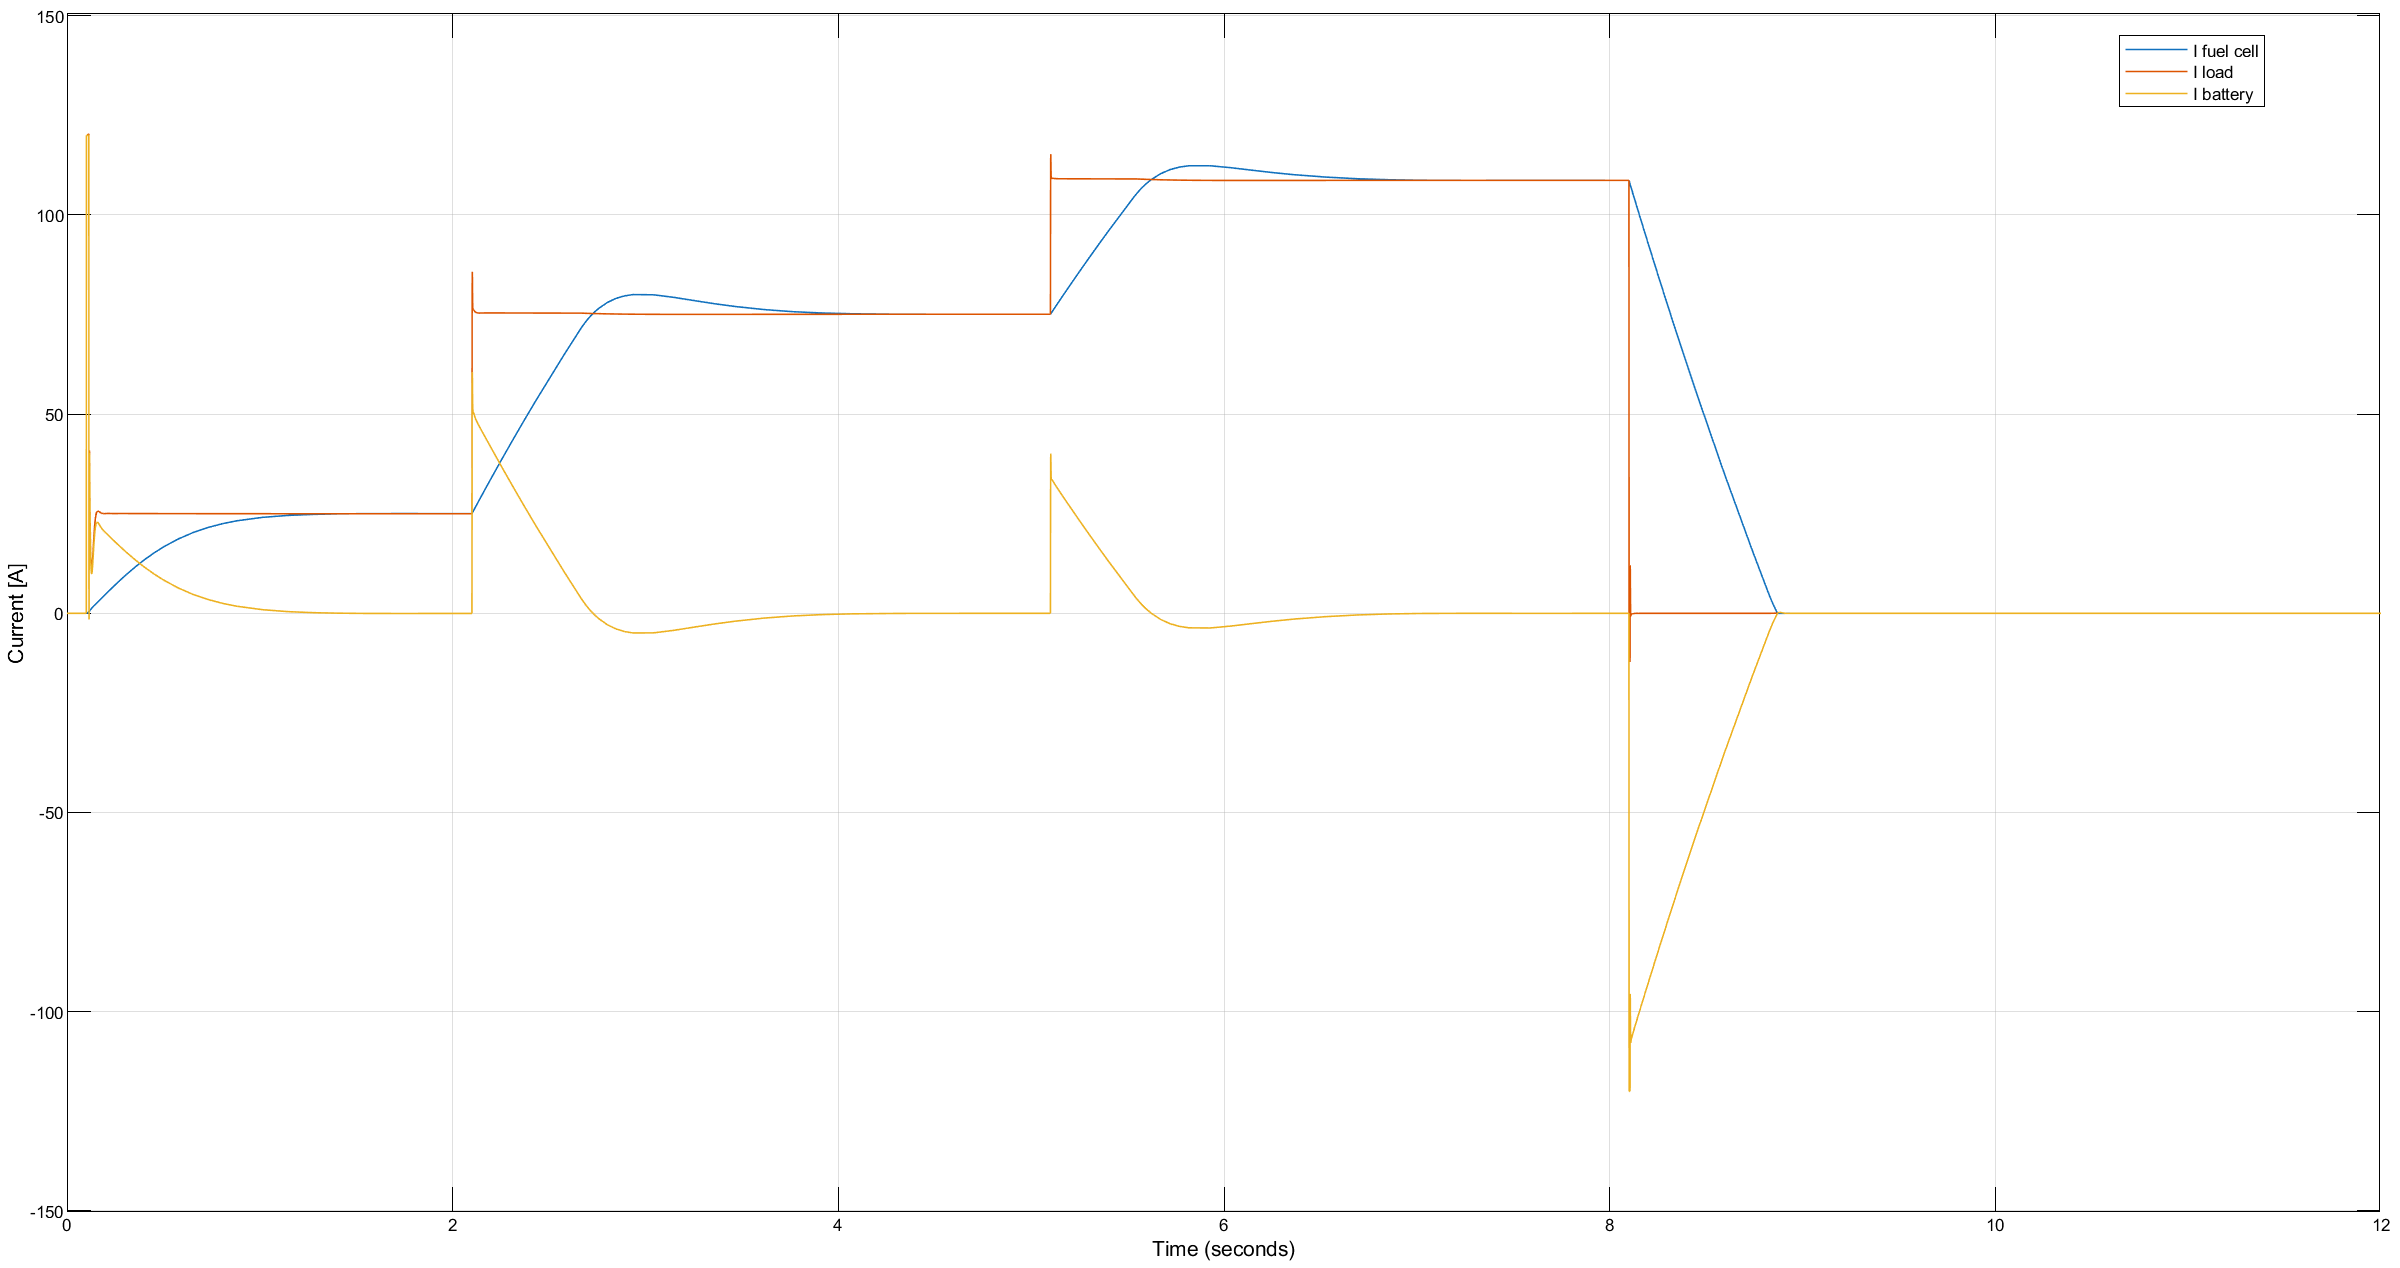
\includegraphics[width=1\linewidth]{img/simulación/i_corrientes_conAWU.png}
    \caption{Corrientes con Anti-WindUp.}
    \label{fig:i_corrientes_conAWU}
\end{figure}

\begin{figure}[H]
    \centering
    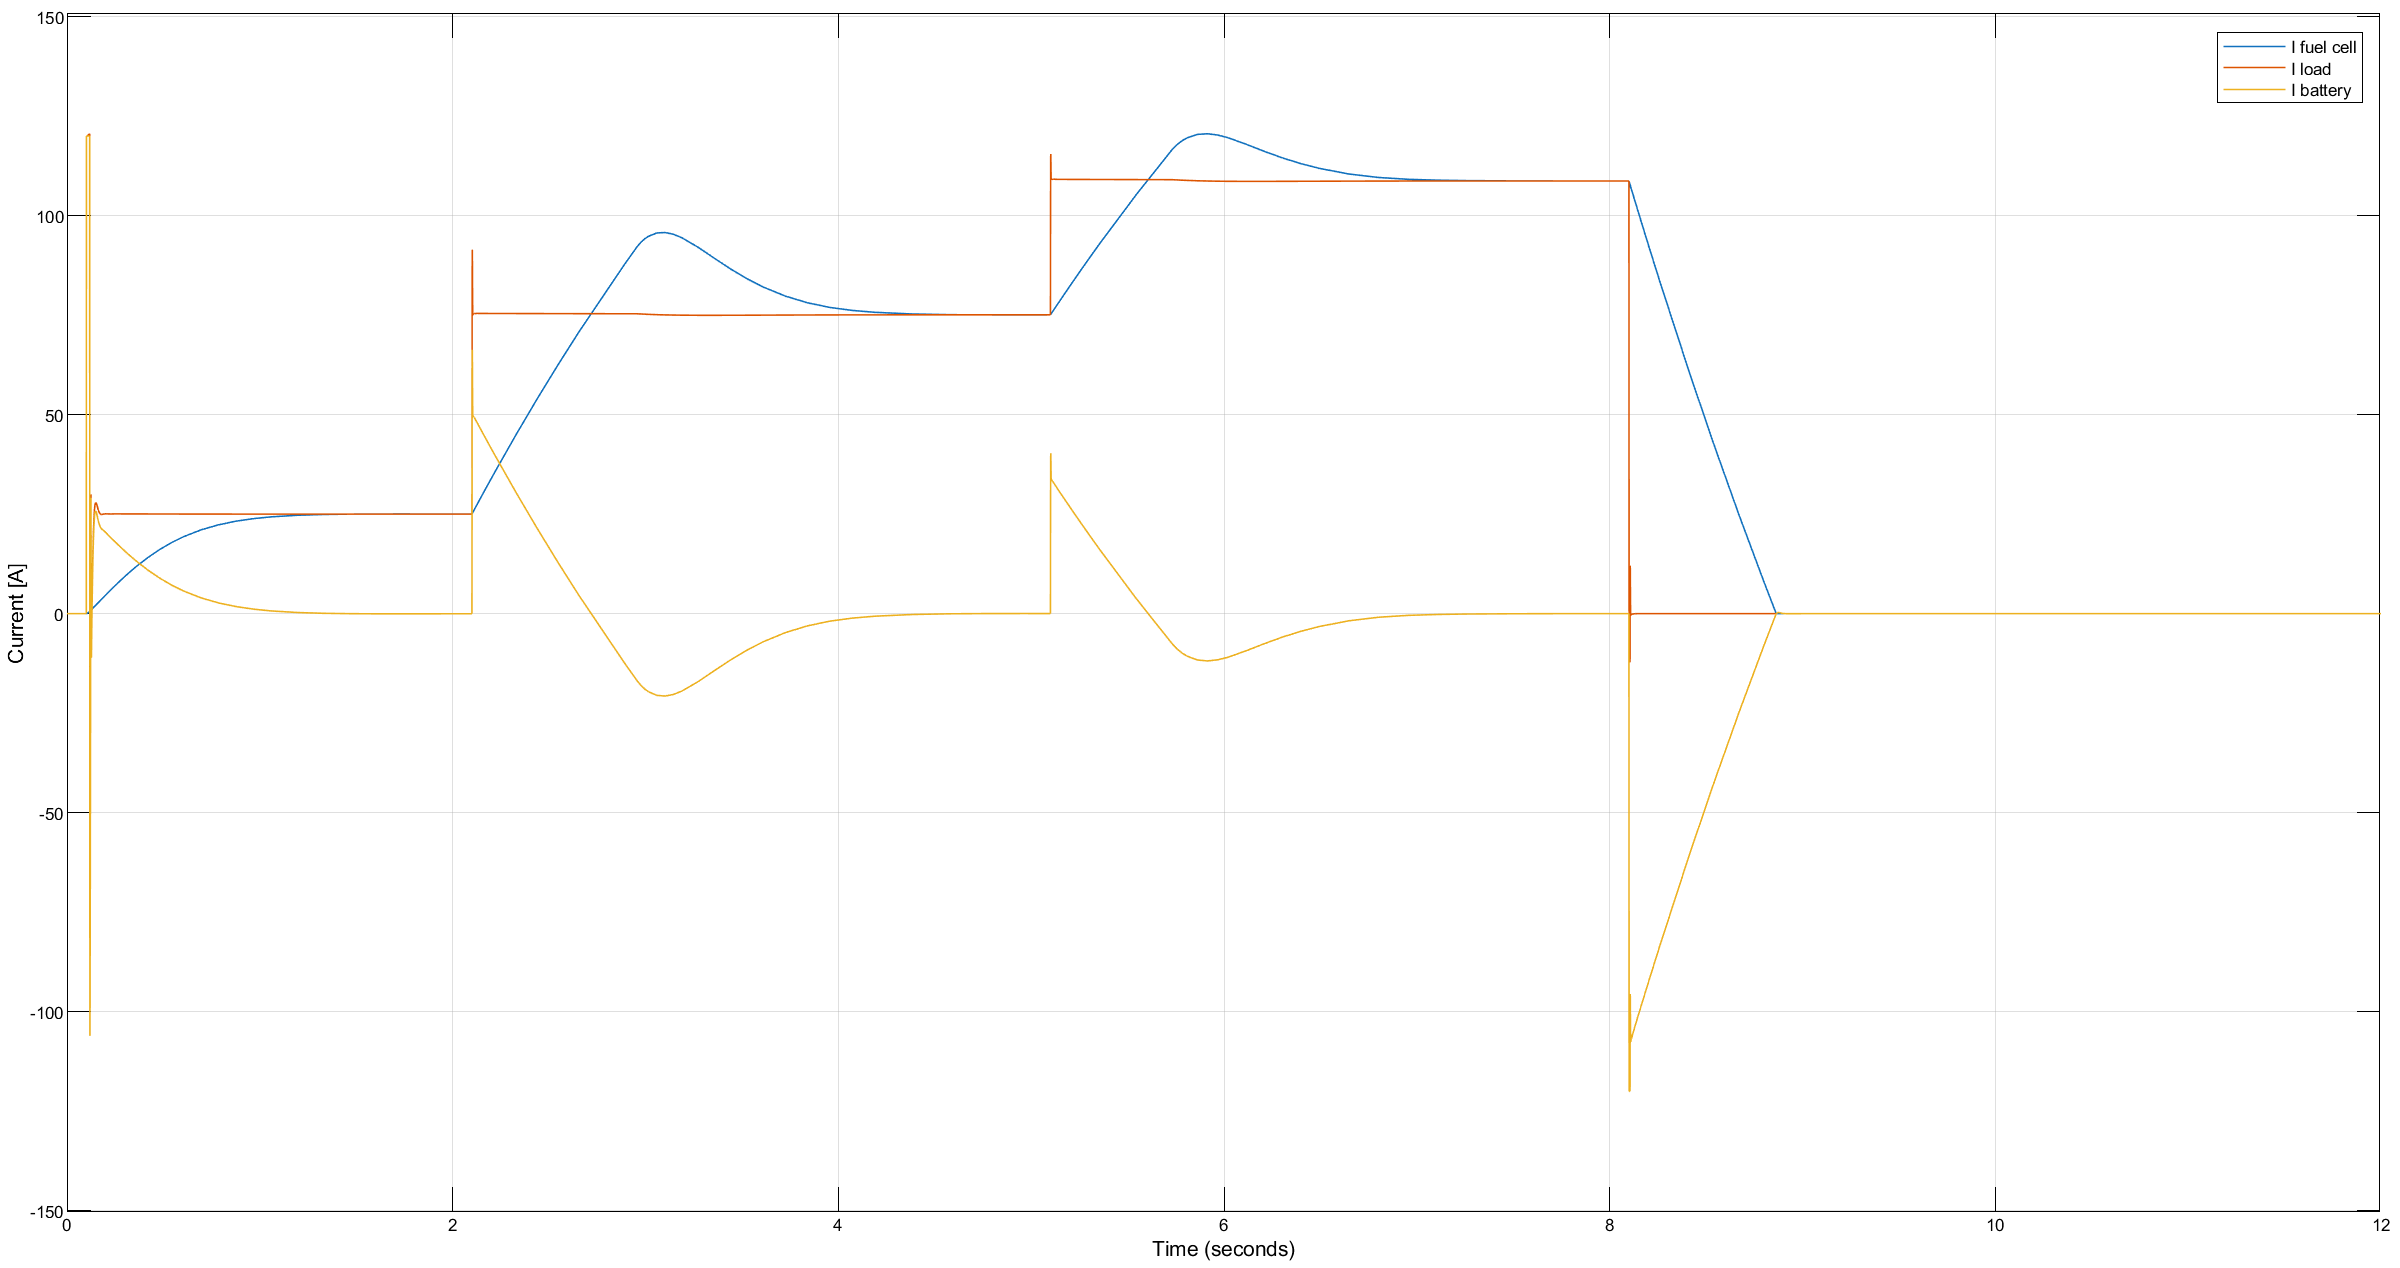
\includegraphics[width=1\linewidth]{img/simulación/i_corrientes_sinAWU.png}
    \caption{Corrientes sin Anti-WindUp.}
    \label{fig:i_corrientes_sinAWU}
\end{figure}

A la hora de la implementación del \textit{feedforward}, se decidió 
analizar el impacto que tiene el \textit{Anti-Windup} en la estrategia de prealimentación.
La diferencia principal se nota en la mejora de las señales de control y la reducción de los sobrepasos de la 
variable controlada. En otras palabras, los actuadores permanecen menos tiempo en la zona de saturación.
Al observar las figuras \ref{fig:i_corrientes_conAWU} y \ref{fig:i_corrientes_sinAWU}
se puede notar que cuando ocurren los eventos de cambio de resistencia $R_L$ las señales de control
tienen sobrepasos mayores cuando el AWU no se encuentra implementado. 

Cuando el sistema carece de AWU el comportamiento dinámico 
muestra una diferencia significativa. Esta diferencia se nota principalmente observando las 
figuras \ref{fig:i_corrientes_sinAWU} y \ref{fig:h_corrientes}.
La distinción de dichas respuestas en principio se nota en la estabilidad de cada sistema. 

\begin{figure}[H]
    \centering
    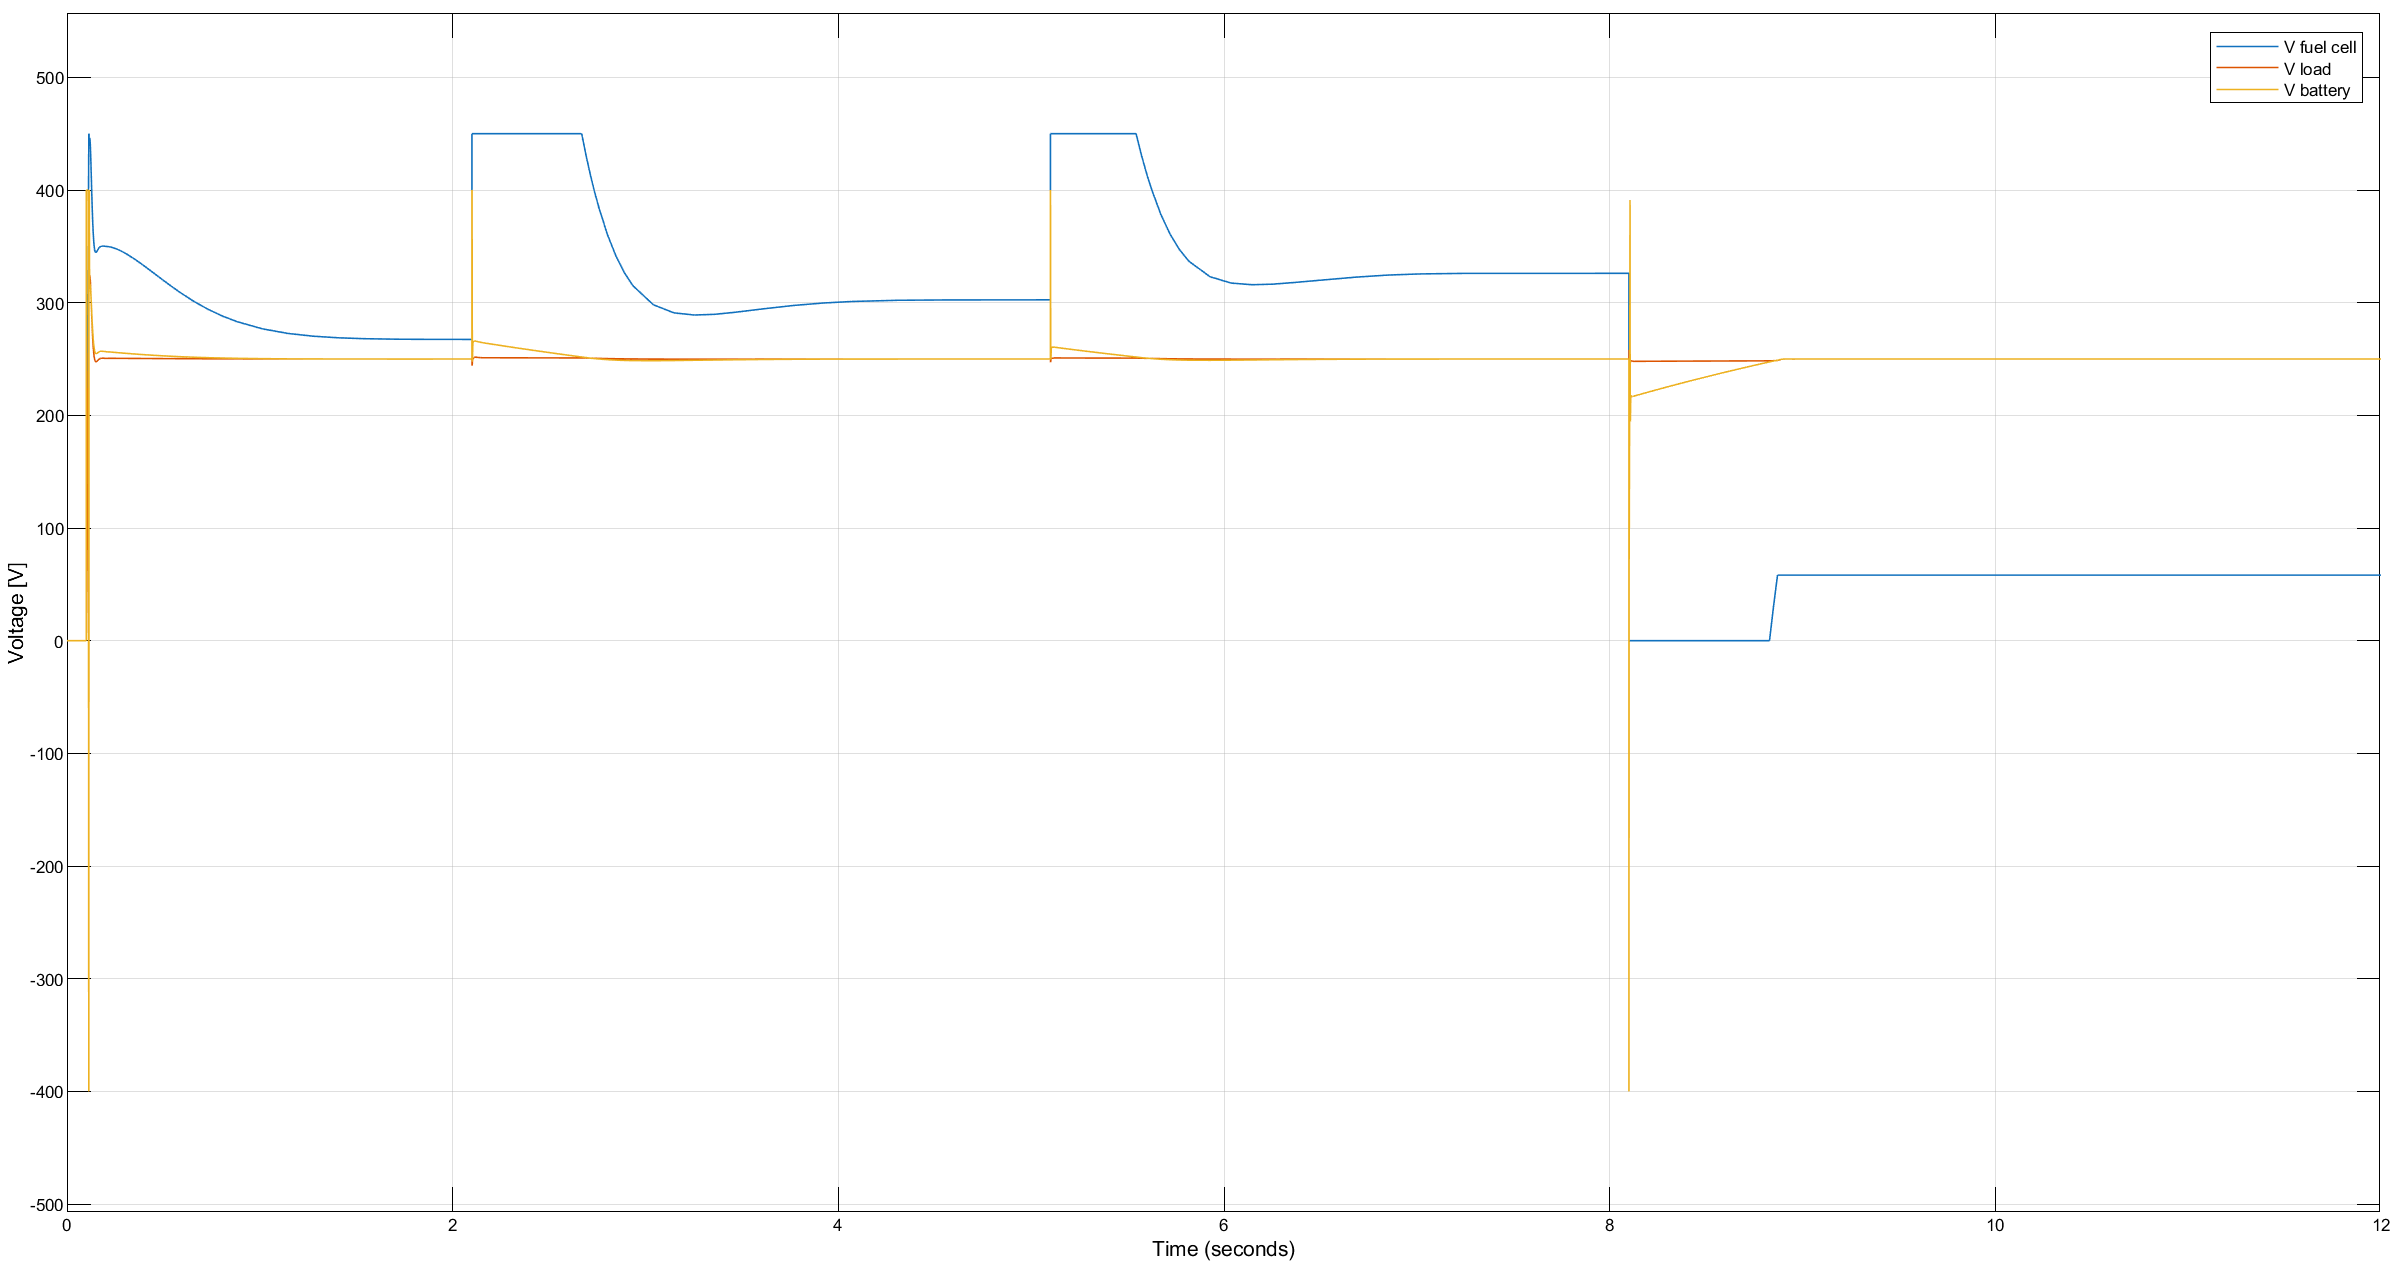
\includegraphics[width=1\linewidth]{img/simulación/i_voltajes_conAWU.png}
    \caption{Voltajes con Anti-WindUp.}
    \label{fig:i_voltajes_conAWU}
\end{figure}

\begin{figure}[H]
    \centering
    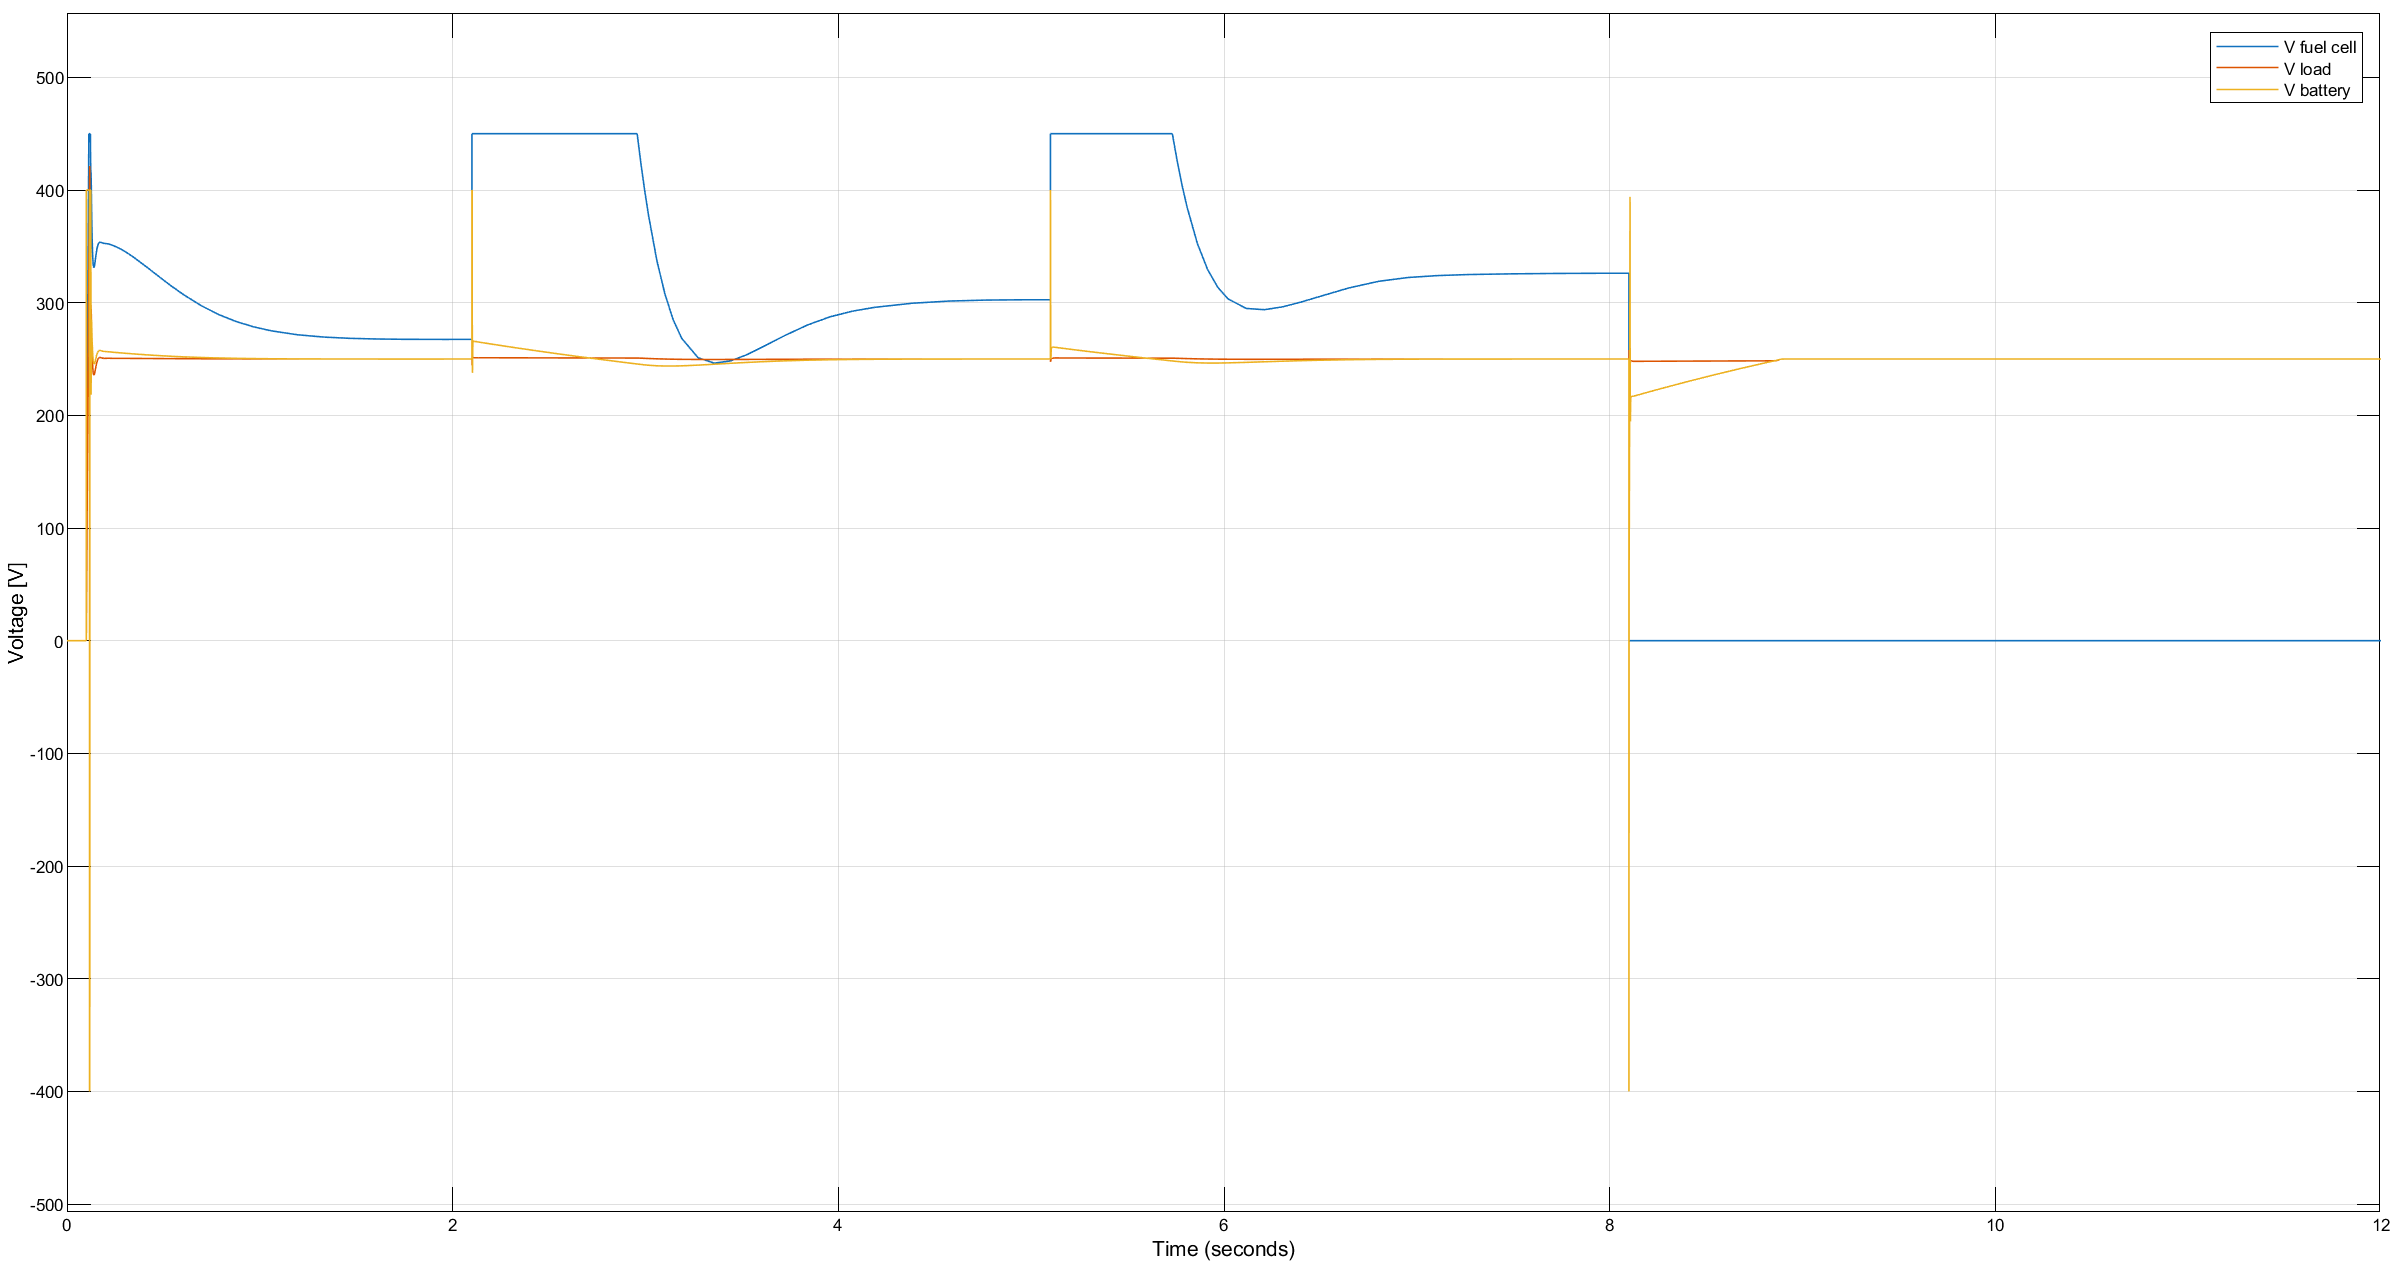
\includegraphics[width=1\linewidth]{img/simulación/i_voltajes_sinAWU.png}
    \caption{Voltajes sin Anti-WindUp.}
    \label{fig:i_voltajes_sinAWU}
\end{figure}

\newpage